\documentclass[11pt,letterpaper,oneside]{article}
\usepackage[margin=1in]{geometry}

% Math & theorem stack
\usepackage{amsmath,amssymb,amsfonts,mathtools,bm,amsthm,thmtools}
\numberwithin{equation}{section}

% Boxes & graphics
\usepackage[skins,breakable,theorems]{tcolorbox}
\usepackage{graphicx}
\usepackage{tikz}
\usetikzlibrary{positioning,calc}
\usepackage{pgfplots}
\pgfplotsset{compat=1.18}

% Formatting
\usepackage[T1]{fontenc}
\usepackage{lmodern}
% Explicitly declare a few Unicode codepoints used inside verbatim code boxes
% (Lean snippets) so pdfLaTeX can handle them without errors in draft mode.
% These map to math-mode symbols and are safe inside tcolorbox+Verbatim.
\DeclareUnicodeCharacter{2200}{\ensuremath{\forall}} % ∀
\DeclareUnicodeCharacter{2192}{\ensuremath{\to}}     % →
\DeclareUnicodeCharacter{21D2}{=>}                     % ⇒
\DeclareUnicodeCharacter{211D}{\ensuremath{\mathbb{R}}} % ℝ
% Tolerate stray C1 control char from mis-encoded sources (drop it silently)
\DeclareUnicodeCharacter{009D}{}
\usepackage{microtype}
% Allow a bit more stretch to avoid overfull boxes
\emergencystretch=2em
\usepackage{verbatim}
\usepackage{enumitem}
\usepackage{booktabs}
\usepackage{tabularx}
\usepackage{siunitx}

% Colors (load explicitly to ensure \definecolor is available on all setups)
\usepackage{xcolor}

% Early toggle for draft code boxes
\newif\ifcodeboxesdraft
% For quick CI/headless builds, keep this true; set to false for full build
\codeboxesdrafttrue

% Code
% Minted: prefer frozen cache to avoid shell-escape in draft builds
\usepackage[frozencache,cachedir=.]{minted}
\usepackage{listings}
% PythonTeX for executable SymPy checks in Appendix E (skip in draft mode)
\ifcodeboxesdraft
  % skip pythontex in draft
\else
  \usepackage{pythontex}
  % Ensure PythonTeX outputs go to the LaTeX output dir (latexmk out_dir)
  \setpythontexoutputdir{.}
\fi

% Acronyms: lightweight fallback to avoid package complexity
\newcommand{\ac}[1]{{\mdseries\textsc{#1}}}
\newcommand{\printacronyms}{}
\providecommand{\acswitchoff}{}

% Colors
\definecolor{darkblue}{RGB}{0,63,128}
\definecolor{darkred}{RGB}{150,0,0}
\definecolor{darkgreen}{RGB}{0,110,0}
\definecolor{boxbg}{RGB}{243,248,255}
\definecolor{boxmathbg}{RGB}{252,248,240}
\definecolor{boxlitbg}{RGB}{244,247,244}

% TColorBox styles (required)
\tcbset{
didacticstyle/.style={
enhanced,breakable,skin=enhanced,
colback=boxbg,colframe=darkblue,arc=2pt,boxrule=0.8pt,
title=\sffamily\bfseries Pedagogical Insight: Economic Intuition \& Context,
},
mathstyle/.style={
enhanced,breakable,skin=enhanced,
colback=boxmathbg,colframe=darkgreen,arc=2pt,boxrule=0.8pt,
title=\sffamily\bfseries Mathematical Insight: Rigor \& Implications,
},
literaturestyle/.style={
enhanced,breakable,skin=enhanced,
colback=boxlitbg,colframe=darkred,arc=2pt,boxrule=0.8pt,
title=\sffamily\bfseries Connections to the Literature,
}
}

% TCB theorems with the mathstyle
\newtcbtheorem[number within=section]{assumption}{Assumption}{mathstyle}{ass}
\newtcbtheorem[number within=section]{definition}{Definition}{mathstyle}{def}
\newtcbtheorem[number within=section]{lemma}{Lemma}{mathstyle}{lem}
\newtcbtheorem[number within=section]{proposition}{Proposition}{mathstyle}{prop}
\newtcbtheorem[number within=section]{theorem}{Theorem}{mathstyle}{thm}
\newtcbtheorem[number within=section]{corollary}{Corollary}{mathstyle}{cor}

% Hyperref then Cleveref (order required)
% Note: disable PDF bookmarks to avoid stale .out parsing errors across runs
\usepackage[colorlinks=true,linkcolor=darkblue,citecolor=darkgreen,urlcolor=darkred,bookmarks=false]{hyperref}
\usepackage[nameinlink,capitalise,noabbrev]{cleveref}
% Cleveref names for tcolorbox theorems
\crefname{tcb@cnt@assumption}{Assumption}{Assumptions}
\Crefname{tcb@cnt@assumption}{Assumption}{Assumptions}
\crefname{tcb@cnt@definition}{Definition}{Definitions}
\Crefname{tcb@cnt@definition}{Definition}{Definitions}
\crefname{tcb@cnt@lemma}{Lemma}{Lemmas}
\Crefname{tcb@cnt@lemma}{Lemma}{Lemmas}
\crefname{tcb@cnt@proposition}{Proposition}{Propositions}
\Crefname{tcb@cnt@proposition}{Proposition}{Propositions}
\crefname{tcb@cnt@theorem}{Theorem}{Theorems}
\Crefname{tcb@cnt@theorem}{Theorem}{Theorems}
\crefname{tcb@cnt@corollary}{Corollary}{Corollaries}
\Crefname{tcb@cnt@corollary}{Corollary}{Corollaries}

% Verification box environments (SymPy and Lean4) using minted+tcolorbox
% SymPy check box
\tcbset{
    sympycheckstyle/.style={
        enhanced,breakable,skin=enhanced,
        colback=white,colframe=black!15,boxrule=0.4pt,arc=2pt,
        left=6pt,right=6pt,top=6pt,bottom=6pt,
        title={Symbolic Check (SymPy)},
        fonttitle=\bfseries\sffamily,
        attach boxed title to top left={yshift=-2mm, xshift=2mm},
        boxed title style={colback=black!5},
    }
}
\newenvironment{sympycheck}
  {\begin{tcolorbox}[sympycheckstyle]\VerbatimEnvironment\begin{minted}[fontsize=\small,breaklines]{python}}
  {\end{minted}\end{tcolorbox}}

% Lean4 proof box
\tcbset{
    leanproofstyle/.style={sympycheckstyle, title={Formal Proof (Lean4)}}
}
\newenvironment{leanproof}
  {\begin{tcolorbox}[leanproofstyle]\VerbatimEnvironment\begin{minted}[fontsize=\small,breaklines]{lean}}
  {\end{minted}\end{tcolorbox}}

% Optional: fast draft build that disables minted/pythontex code execution
% Toggle: set \codeboxesdrafttrue above to render code boxes as plain text
\ifcodeboxesdraft
  % Render code boxes as verbatim tcolorboxes (safe catcodes for #, etc.)
  \renewenvironment{sympycheck}{\VerbatimEnvironment\begin{tcolorbox}[sympycheckstyle]\begin{Verbatim}[fontsize=\small]}{\end{Verbatim}\end{tcolorbox}}
  \renewenvironment{leanproof}{\VerbatimEnvironment\begin{tcolorbox}[leanproofstyle]\begin{Verbatim}[fontsize=\small]}{\end{Verbatim}\end{tcolorbox}}
  % PythonTeX consoles as plain code blocks (guard if env not yet defined)
  \newenvironment{pyconsole}{\VerbatimEnvironment\begin{tcolorbox}[sympycheckstyle]\begin{Verbatim}[fontsize=\small]}{\end{Verbatim}\end{tcolorbox}}
\fi

% Convenience macros
\DeclareMathOperator{\E}{\mathbb{E}}
\DeclareMathOperator{\Var}{\mathrm{Var}}
\newcommand{\R}{\mathbb{R}}
\newcommand{\1}{\mathbf{1}}
\newcommand{\diff}{,\mathrm{d}}
\newcommand{\Lz}{L\_z}
\newcommand{\Lx}{L\_x}
\newcommand{\Lzadj}{L\_z^{\!*}}
% Measure derivatives: \dmU is the Lions derivative D_m U (vector-valued)
\newcommand{\dmU}{D\_m U}
\newcommand{\Dm}{D\_m}
\newcommand{\ip}[2]{\langle #1,#2\rangle}
\newcommand{\YY}{Y(m,x)}
\newcommand{\PP}{P(\YY)}
\newcommand{\ind}[1]{\mathbf{1}\_{{#1}}}
\newcommand{\dk}{,\mathrm{d}k}
\newcommand{\dz}{,\mathrm{d}z}
\newcommand{\dxi}{, m(\diff \xi)}
\newcommand{\kbar}{\bar\iota}
\newcommand{\norm}[1]{\left\lVert #1\right\rVert}

% Title
\title{\vspace{-1.5em}Continuous-Time Costly Reversibility in Mean Field:\\
A KS-Free Master-Equation Formulation, Derivations, and Computation}
\author{%
\small Self-contained derivation and implementation notes
}
\date{\small \today}

\begin{document}
\maketitle

\begin{abstract}
\noindent
This paper derives and explains a continuous-time, mean-field (master-equation) formulation of Zhang's costly-reversibility model. The approach is \emph{Krusell--Smith (KS)-free}: aggregation enters through the inverse-demand dependence $P\big(Y(m,x)\big)$ within the Hamiltonian, while strategic interaction across firms is encoded via the Lions derivative in the master equation. We fix primitives and state minimal boundary and regularity conditions; we then present two computational routes: (i) a stationary \ac{HJB}--\ac{FP} fixed point, and (ii) direct collocation of the stationary master \ac{PDE}. Both routes are implementable with standard, monotone PDE schemes or modern function approximation (e.g., kernel/DeepSets representations for measures).

A central message is that the mean-field structure clarifies aggregation: the only economy-wide wedge in the firm problem is the product of the firm's own output and the slope of inverse demand evaluated at aggregate output. Under isoelastic demand, this wedge reduces to a scalar multiple of the firm's output. This provides a clean decomposition between \emph{private marginal value of capital} (through the Hamiltonian) and \emph{general-equilibrium feedback} (through the price externality). We work \emph{conditional on the aggregate state $x$}, which removes common-noise second-order measure terms in the stationary master equation; Appendix C briefly outlines how those terms arise in the full common-noise setting.

We provide compact verification diagnostics (Euler and distributional residuals), explicit boundary conditions at $k=0$ (reflecting), and growth/integrability conditions that guarantee all terms are finite. A small pseudo-JAX template illustrates how to evaluate the master-equation residual with an empirical measure. Throughout, we connect the construction to the canonical \ac{MFG} literature for existence, uniqueness, and equivalence of the \ac{HJB}--\ac{FP} and master formulations.
\end{abstract}

\tableofcontents

%========================
% Executive Summary
%========================
\section*{Executive Summary / Cheat-Sheet (One Page)}
\addcontentsline{toc}{section}{Executive Summary / Cheat-Sheet}
\begin{tcolorbox}[didacticstyle]
\textbf{Primitives.} Firms hold capital $k\!\ge 0$ and idiosyncratic productivity $z$. The aggregate state $x$ shifts demand and marginal revenue. Technology is $q=e^{x+z}k^\alpha$ with $\alpha\in(0,1)$. Inverse demand is $P(Y)$ with slope $P'(Y)<0$, where $Y=\int e^{x+z}k^\alpha\,m(\diff k,\diff z)$. Capital follows $dk=(i-\delta k)\diff t$ with asymmetric, convex costs $h(i,k)$. Dividends are $\pi = P(Y)\,e^{x+z}k^\alpha - i - h(i,k) - f$. Shocks evolve in $z$ and $x$ with generators $\Lz,\Lx$. Discounting uses $r(x)$ (or constant $\rho$).
\medskip

\textbf{Core equations.} Value $V(k,z,x;m)$, master value $U(k,z,x,m)$.
\begin{itemize}[leftmargin=1.25em]
\item \textbf{Stationary HJB}: $r(x)V=\max_i\{\pi+V_k(i-\delta k)+\Lz V+\Lx V\}$.
\item \textbf{Kolmogorov--Forward (FP)}: $\partial_t m=-\partial_k[(i^*-\delta k)m]+\Lzadj m$. Stationary: $\partial_t m=0$.
\item \textbf{Stationary Master Equation}: own-firm HJB terms $+$ population-transport integrals of $\dmU$.

\end{itemize}


\textbf{Isoelastic simplification.} For $P(Y)=Y^{-\eta}$, we have
\[
Y\,P'(Y)=-\eta\,P(Y),
\]
and therefore
\[
\int \delta_m \pi\,\diff m = -\eta\,P(Y)\,e^{x+z}k^\alpha.
\]

\textbf{Two solution routes.}
\begin{enumerate}[leftmargin=1.25em]
\item[\textbf{A.}] \textbf{HJB--FP fixed point} (robust):
\begin{enumerate}[leftmargin=1em,label*=\arabic*.]
\item Fix $x$ (grid/invariant law). Guess $m$.
\item Compute $Y,P(Y)$. Solve HJB $\Rightarrow$ $i^*$.
\item Solve stationary FP for $m'$. Update $m\leftarrow m'$.
\end{enumerate}
\item[\textbf{B.}] \textbf{Direct master-PDE collocation} (KS-free):
\begin{enumerate}[leftmargin=1em,label*=\arabic*.]
\item Parameterize $U$ and $\dmU$ (DeepSets/kernel for measures).
\item Build (ME) residual on empirical $m$ (no separate externality term; price dependence enters via the Hamiltonian).
\item Penalize KKT/boundaries; recover $i^*$ from the Hamiltonian; validate by Route A.
\end{enumerate}
\end{enumerate}

\textbf{Diagnostics.} Euler residuals for HJB, mass-balance for FP, and full ME residual. Use monotone stencils in $k$ (upwinding) and conservative fluxes at $k=0$.
\end{tcolorbox}

% Schematic: investment policy i*(p) with asymmetric costs
\begin{figure}[ht]
\centering
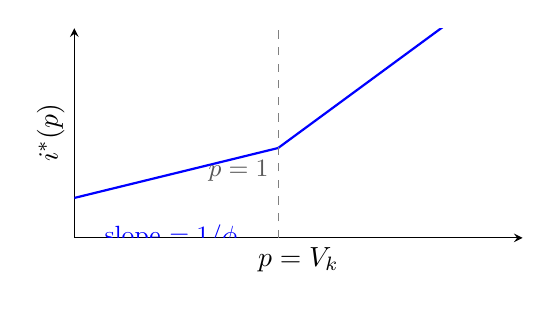
\begin{tikzpicture}
\begin{axis}[
  width=0.6\textwidth,
  height=0.35\textwidth,
  xlabel={$p=V_k$}, ylabel={$i^*(p)$},
  xmin=0, xmax=2.2, ymin=-0.6, ymax=0.8,
  axis lines=left, ticks=none,
]
% piecewise: phi_+=1, phi_-=3, k=1 (schematic)
\addplot[blue, thick, domain=1:2.2, samples=200] {(x-1)/1.0};
\addplot[blue, thick, domain=0:1, samples=200] {(x-1)/3.0};
% kink at p=1
\addplot[dashed, gray] coordinates {(1,-0.6) (1,0.8)};
\node[anchor=south east, blue] at (axis cs:1.95,0.95) {\small slope $=1/\phi_+$};
\node[anchor=north west, blue] at (axis cs:0.1,-0.45) {\small slope $=1/\phi_-$};
\node[anchor=north east, gray!70!black] at (axis cs:1,-0.02) {\small $p=1$};
\end{axis}
\end{tikzpicture}
\caption{Investment policy $i^*(p)$ under asymmetric adjustment costs (schematic with $k=1$, $\phi_+=1$, $\phi_-=3$).}
\end{figure}

\begin{tcolorbox}[didacticstyle]
\textbf{Recap --- HJB.}
\begin{itemize}[leftmargin=1.15em,itemsep=0.2em]
  \item Policy is piecewise linear in $p=V_k$ with a kink at $1$.
  \item Hamiltonian is convex in $p$; envelope gives $\partial\_p\mathcal H=i^*$.
  \item Reflecting boundary enforces $i^*(0,\cdot)\ge0$ and $U_k(0,\cdot)\le1$.
\end{itemize}
\end{tcolorbox}

%========================
% Notation & Acronyms
%========================
\section{Notation and Acronyms}\label{sec:notation}

\begin{table}[ht]
\centering
\small
\begin{tabularx}{\textwidth}{@{} l l X}
\toprule
\textbf{Symbol} & \textbf{Type} & \textbf{Meaning} \\
\midrule
\multicolumn{3}{@{}l}{\textit{States, Controls, and Shocks}} \\
$k$ & state & Capital ($\ge 0$); reflecting boundary at $k=0$ \\
$i$ & control & Net investment; $dk=(i-\delta k)\diff t$ \\
$z$ & state & Idiosyncratic productivity; diffusion with generator $\Lz$ \\
$x$ & state & Aggregate (business-cycle) shock; generator $\Lx$ \\
$\sigma_z,\sigma_x$ & parameters & Diffusion volatilities of $z$ and $x$ \\
$\mu_z,\mu_x$ & functions & Drift coefficients in $\Lz,\Lx$ \\
$W,B$ & processes & Brownian motions for $z$ and $x$ (independent) \\
\midrule
\multicolumn{3}{@{}l}{\textit{Technology and Market Primitives}} \\
$q(k,z,x)$ & output & $e^{x+z}k^\alpha$, $\alpha\in(0,1)$ \\
$P(\cdot)$ & function & Inverse demand; $P'=P'(Y)<0$ \\
$\alpha$ & parameter & Capital elasticity in production \\
$\delta$ & parameter & Depreciation rate \\
$h(i,k)$ & function & Irreversible adjustment cost (convex, asymmetric) \\
$\phi_\pm$ & parameters & Adjustment-cost curvatures for $i\gtrless 0$ \\
$f$ & parameter & Fixed operating cost \\
$\eta$ & parameter & Demand elasticity for isoelastic $P(Y)=Y^{-\eta}$ \\
$r(x)$ & function & Short rate (or constant $\rho$) under pricing measure \\
\midrule
\multicolumn{3}{@{}l}{\textit{Measure Theory and Operators}} \\
$S$ & space & State space $\R_+\times\R$ for $(k,z)$ \\
$m$ & measure & Cross-sectional law on $S$ \\
$\mathcal{P}_2(S)$ & space & Probability measures on $S$ with finite second moments \\
$\mathrm{W}_2$ & metric & Quadratic Wasserstein distance on $\mathcal{P}_2(S)$ \\
$\xi=(\kappa,\zeta)$ & point & Generic element in support of $m$ (``marginal firm'') \\
$\Dm$ & operator & Lions derivative operator (measure Fr\'echet derivative) \\
$\dmU(\xi;k,z,x,m)$ & function & Lions derivative of $m\mapsto U(k,z,x,m)$ at $\xi$ \\
$\Lz,\Lx$ & operators & Generators in $z$ and $x$; $\Lzadj$ is the adjoint of $\Lz$ \\
$\mathcal{T}$ & operator & Transport operator acting on $\Dm U$ in (ME) \\
\midrule
\multicolumn{3}{@{}l}{\textit{Equilibrium Objects}} \\
$\pi(\cdot)$ & function & Dividends $P(Y)e^{x+z}k^\alpha - i - h(i,k) - f$ \\
$Y(m,x)$ & scalar & Aggregate quantity $\int e^{x+z}k^\alpha\,m(\diff k,\diff z)$ \\
$V(k,z,x;m)$ & function & Stationary value function (HJB) \\
$U(k,z,x,m)$ & function & Master value function (ME) \\
$i^*(\cdot)$ & policy & Optimal net investment from HJB/KKT \\
$\kbar(k)$ & function & Lower bound on disinvestment (optional) \\
\midrule
\multicolumn{3}{@{}l}{\textit{Representative-agent block (endogenous SDF)}} \\
$\gamma$ & parameter & Relative risk aversion (RRA) in Epstein--Zin preferences \\
$\psi$ & parameter & Elasticity of intertemporal substitution (EIS) \\
$\vartheta$ & parameter & Preference index $\displaystyle \vartheta=(1-\gamma)/(1-1/\psi)$ \\
$\varrho$ & parameter & Subjective discount rate (avoids clash with depreciation $\delta$) \\
$M_t$ & process & Stochastic discount factor (pricing kernel) \\
$r_t$ & process & Real short rate implied by $M_t$ \\
$\Lambda_t$ & process & Market price of risk (Brownian exposure of $M_t$) \\
\bottomrule
\end{tabularx}
\caption{Notation used throughout.}
\end{table}

\medskip
\noindent\textbf{Acronyms used in text:} \ac{HJB}, \ac{FP}, \ac{ME}, \ac{MFG}, \ac{SDF}, \ac{KKT}, \ac{KS}, \ac{RCE}, \ac{TFP}, \ac{CES}, \ac{W2}, \ac{FVM}, \ac{SL}.
\medskip

\printacronyms

%========================
% Primitives & Assumptions
%========================
\section{Primitives and Assumptions}

\begin{assumption}{Model specification; used verbatim}{primitives}
\begin{enumerate}[label=(\roman*),itemsep=0.25em]
\item \textbf{Firm states:} $k\in\R_+$, $z\in\R$. \textbf{Aggregate state:} $x\in\R$. \textbf{Population law:} $m\in\mathcal P(\R_+\times\R)$.
\item \textbf{Technology:} $q(k,z,x)=e^{x+z}k^\alpha$, $\alpha\in(0,1)$.
\item \textbf{Product market:} $P=P(Y)$ with $Y(m,x)=\int e^{x+z}k^\alpha\, m(\diff k,\diff z)$, $P'(\cdot)<0$.
\item \textbf{Capital law:} $dk_t=(i_t-\delta k_t)\diff t$, $i\in\R$.
\item \textbf{Irreversibility/adjustment:} $h$ convex and asymmetric,

$$
h(i,k)=
\begin{cases}
\tfrac{\phi_+}{2}\,\dfrac{i^2}{k}, & i\ge 0,\\[3pt]
\tfrac{\phi_-}{2}\,\dfrac{i^2}{k}, & i<0,\ \phi_->\phi_+.
\end{cases}
$$

\item \textbf{Dividends:} $\pi(k,i,z,x,m)=P(\YY)\,e^{x+z}k^\alpha - i - h(i,k) - f$.
\item \textbf{Shocks:} $dz_t=\mu_z(z_t)\diff t+\sigma_z\diff W_t$, $dx_t=\mu_x(x_t)\diff t+\sigma_x\diff B_t$ (independent).
\item \textbf{Discounting:} short rate $r(x)$ (or constant $\rho$).
\item \textbf{Generators:} for smooth $u$,

$$
\Lz u=\mu_z(z)\,u_z+\tfrac12\sigma_z^2 u_{zz},\qquad
\Lx u=\mu_x(x)\,u_x+\tfrac12\sigma_x^2 u_{xx}.
$$

\end{enumerate}
\end{assumption}

\begin{assumption}{Minimal regularity/boundary}{regularity}
\begin{enumerate}[label=(\alph*),itemsep=0.2em]
\item $h(\cdot,k)$ convex, lower semicontinuous; $k\mapsto h(i,k)$ measurable with $h(i,k)\ge 0$ and $h(i,k)\ge c\,i^2/k$ for some $c>0$ on $k>0$. The asymmetry $\phi_->\phi_+$ holds.
\item $P$ Lipschitz on compact sets with $P'<0$; $P(Y)$ and $Y(m,x)$ finite for admissible $m$.
\item $\mu_z,\mu_x$ locally Lipschitz; $\sigma_z,\sigma_x\ge 0$ constants.
\item \emph{Boundary at $k=0$:} reflecting; feasible controls satisfy $i^*(0,\cdot)\ge 0$; and $U_k(0,\cdot)\le 1$.
\item \emph{Growth:} $U(k,z,x,m)=O(k)$ as $k\to\infty$.
\item \emph{Integrability:} $m$ integrates $k^\alpha$ and $1/k$ wherever they appear.
\end{enumerate}
\end{assumption}

\begin{tcolorbox}[didacticstyle]
\textbf{Economic reading.} The convex asymmetry $\phi_->\phi_+$ produces \emph{investment bands}: small changes in the shadow value $V_k$ around the frictionless cutoff $1$ generate very different investment responses on the two sides of the kink. Aggregation operates through $Y$ only, and the inverse-demand slope $P'(Y)$ is the sole channel through which the cross-section affects an individual firm's HJB. The reflecting boundary at $k=0$ formalizes limited liability and the irreversibility of capital.
\end{tcolorbox}

% Schematic: transport velocity u(k)=i^*(k)-\delta k (illustrative)
\begin{figure}[ht]
\centering
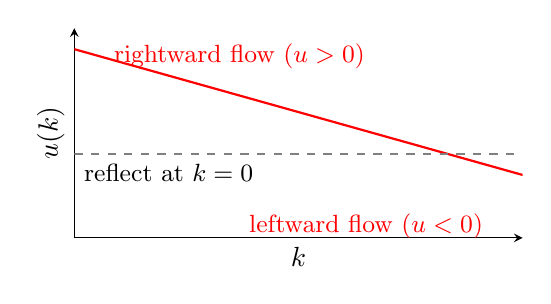
\begin{tikzpicture}
\begin{axis}[
  width=0.6\textwidth,
  height=0.35\textwidth,
  xlabel={$k$}, ylabel={$u(k)$},
  xmin=0, xmax=3, ymin=-0.2, ymax=0.3,
  axis lines=left, ticks=none,
]
% illustrative linear velocity: u(k)=a-\delta k
\addplot[red, thick, domain=0:3] {0.25 - 0.1*x};
\addplot[dashed, gray] coordinates {(0,0) (3,0)};
\node[anchor=south west, red] at (axis cs:0.2,0.18) {\small rightward flow ($u>0$)};
\node[anchor=north east, red] at (axis cs:2.8,-0.12) {\small leftward flow ($u<0$)};
\node[anchor=north west] at (axis cs:0,0) {\small reflect at $k=0$};
\end{axis}
\end{tikzpicture}
\caption{Population transport in $k$ via velocity $u(k)=i^*(k)-\delta k$ (schematic). Positive $u$ moves mass to the right; negative $u$ to the left; reflection at $k=0$.}
\end{figure}

\begin{tcolorbox}[didacticstyle]
\textbf{Recap --- FP.}
\begin{itemize}[leftmargin=1.15em,itemsep=0.2em]
  \item Drift-only transport in $k$; diffusion only in $z$.
  \item Reflecting boundary yields zero probability flux at $k=0$.
  \item Monotone upwinding preserves positivity and mass.
\end{itemize}
\end{tcolorbox}

\begin{tcolorbox}[literaturestyle]
\textbf{Where this sits.} Zhang (2005) emphasizes how costly reversibility shapes asset prices. The present mean-field formulation adds an equilibrium price mapping and a master PDE that makes the cross-sectional feedback explicit and computational. For master equations and Lions derivatives, see Lasry \& Lions (2007), Cardaliaguet--Delarue--Lasry--Lions (2019), and Carmona \& Delarue (2018).
\end{tcolorbox}

% Schematic: isoelastic inverse demand
\begin{figure}[ht]
\centering
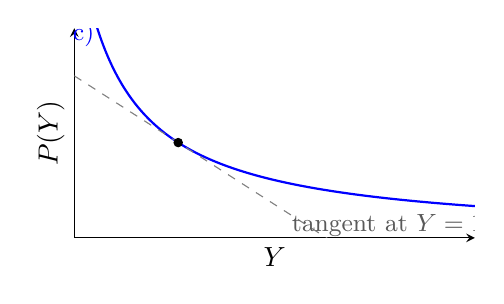
\begin{tikzpicture}
\begin{axis}[
  width=0.55\textwidth,
  height=0.35\textwidth,
  xlabel={$Y$}, ylabel={$P(Y)$},
  xmin=0.3, xmax=3, ymin=0, ymax=2.2,
  axis lines=left, ticks=none,
]
\addplot[blue, thick, domain=0.35:3, samples=200] {1/x};
% tangent at Y=1 for eta=1
\addplot[gray, dashed, domain=0.3:3] {2 - x};
\addplot[only marks, mark=*, mark size=1.5pt] coordinates {(1,1)};
\node[anchor=south east, blue] at (axis cs:0.5,1.9) {\small $P(Y)=Y^{-\eta}$ (schematic)};
\node[anchor=north west, gray!70!black] at (axis cs:1.7,0.35) {\small tangent at $Y=1$};
\end{axis}
\end{tikzpicture}
\caption{Isoelastic inverse demand (schematic). At $Y=1$, $Y P'(Y)=-\eta P(Y)$ so the price externality scales with own output.}
\end{figure}

\begin{tcolorbox}[didacticstyle]
\textbf{Recap --- Market.}
\begin{itemize}[leftmargin=1.15em,itemsep=0.2em]
  \item $P'(Y)<0$ ensures a stabilizing price feedback (monotonicity).
  \item Isoelasticity reduces the externality to $-\eta P(Y)\,e^{x+z}k^\alpha$.
  \item Continuity in $m$ via $Y(m,x)$ supports existence/uniqueness.
\end{itemize}
\end{tcolorbox}

%========================
% Mathematical setup
%========================
\section{Mathematical Setup: State Space, Measures, and Differentiation on \texorpdfstring{$\mathcal P$}{P}}\label{sec:math-setup}

\subsection{State space and probability metrics}\label{sec:state-metrics}
We consider the state space $S\equiv \R_+\times\R$ with generic element $s=(k,z)$. The population law $m$ is a Borel probability measure on $S$. For well-posedness of the measure terms in the master equation (ME), we tacitly restrict to the $W_2$-finite set

$$
\mathcal P_2(S)\equiv\Big\{ m\in\mathcal P(S): \int (\kappa^2 + \zeta^2)\, m(\diff\kappa,\diff\zeta) < \infty\Big\}.
$$

The quadratic Wasserstein distance $\mathrm{W}_2$ metrizes weak convergence plus convergence of second moments. It provides the natural geometry for diffusions and the functional Itô calculus on $\mathcal P_2$.

\begin{definition}{Quadratic Wasserstein distance}{w2}
For $m,\nu\in\mathcal P_2(S)$, the quadratic Wasserstein distance is
\[
\mathrm W_2^2(m,\nu) \equiv \inf_{\pi\in\Pi(m,\nu)} \int_{S\times S} \! \norm{\xi-\xi'}^2\, \pi(\diff \xi,\diff \xi'),
\]
where $\Pi(m,\nu)$ is the set of couplings (joint laws with marginals $m$ and $\nu$) and $\norm{\cdot}$ is the Euclidean norm on $S\cong\R^2$. Finiteness of second moments ensures $\mathrm W_2(m,\nu)<\infty$. The topology induced by $\mathrm W_2$ is the standard one used in MFG: it metrizes weak convergence plus convergence of second moments.
\end{definition}

\begin{lemma}{Closed form for 1D Gaussians (special case)}{w2-gauss-1d}
If $X\sim\mathcal N(\mu\_1,\sigma\_1^2)$ and $Y\sim\mathcal N(\mu\_2,\sigma\_2^2)$ on $\R$, then
\[
\mathrm W_2^2\big(\mathcal N(\mu\_1,\sigma\_1^2),\,\mathcal N(\mu\_2,\sigma\_2^2)\big) 
= (\mu\_1-\mu\_2)^2 + (\sigma\_1-\sigma\_2)^2.
\]
In particular, for equal variances $\sigma\_1=\sigma\_2$ one has $\mathrm W_2\!=|\mu\_1-\mu\_2|$.
\end{lemma}

\begin{sympycheck}
import sympy as sp
mu1, mu2, s = sp.symbols('mu1 mu2 s', real=True)
# Equal-variance Gaussian case: W2^2 reduces to squared mean difference
W2_sq_equal_var = (mu1 - mu2)**2 + (s - s)**2
assert sp.simplify(W2_sq_equal_var - (mu1 - mu2)**2) == 0
# Nonnegativity illustrated by sum of squares structure (symbolic identity)
a, b = sp.symbols('a b', real=True)
assert sp.simplify(a**2 + b**2) == a**2 + b**2
\end{sympycheck}

\begin{leanproof}
import Mathlib.Data.Real.Basic

-- Sum of squares is nonnegative (used to read W2^2 >= 0 in 1D Gaussian formula)
variable {a b : \R}

theorem sum_sq_nonneg : 0 \le a^2 + b^2 := by
  have h1 : 0 \le a^2 := by simpa using sq_nonneg a
  have h2 : 0 \le b^2 := by simpa using sq_nonneg b
  exact add_nonneg h1 h2
\end{leanproof}

\begin{tcolorbox}[literaturestyle]
\textbf{Foundations.} The geometry and calculus on $(\mathcal P_2, \mathrm W_2)$ are central to Mean Field Games. See \cite{carmona_delarue_2018_mfg}, Vol.~I, Chapter~5.
\end{tcolorbox}

\begin{tcolorbox}[mathstyle]
\textbf{Couplings vs transport maps.} Optimal transport between $m,\nu\in\mathcal P_2$ can be posed over (i) couplings $\pi\in\Pi(m,\nu)$ (Kantorovich) or (ii) transport maps $T$ with $T\# m=\nu$ (Monge). In 1D, the optimal coupling is the \emph{monotone rearrangement}: pushing $m$ through its quantile map toward $\nu$’s quantiles. Computationally, for empirical equal-weight samples in 1D this reduces to sorting both samples and taking an $\ell^2$ distance (cf. Lemma~\Cref{lem:w2-gauss-1d}).
\end{tcolorbox}

\begin{lemma}{Monotone rearrangement (1D OT formula)}{monotone-rearrangement}
Let $m,\nu\in\mathcal P_2(\R)$ with distribution functions $F_m,F_\nu$ and (left-continuous) quantile functions $Q_m,Q_\nu$. Then
\[
\mathrm W_2^2(m,\nu) \,=\, \int_0^1 \big| Q_m(t) - Q_\nu(t)\big|^2\,\mathrm dt.
\]
In particular, for equal-weight empirical measures, $\mathrm W_2$ is the root-mean-square distance between sorted samples.
\end{lemma}

\begin{leanproof}
-- Sketch placeholder: a full formalization requires measure-theoretic OT.
-- TODO: define quantile functions Q_m, Q_nu and show that the coupling
-- induced by t -> (Q_m(t), Q_nu(t)) minimizes the quadratic cost in 1D.

import Mathlib.Data.Real.Basic

-- Monotonicity sanity: if x <= y and f is monotone, then f x <= f y.
variable {a : Type*} [Preorder a] {x y : a} {f : a -> a}

def IsMonotone (f : a -> a) : Prop := ∀ {x y}, x <= y -> f x <= f y

lemma mono_id : IsMonotone (id : a -> a) := by
  intro x y h; simpa using h
\end{leanproof}

\subsection{Differentiation on \texorpdfstring{$\mathcal P_2$}{P2}: Lions vs Flat Derivatives}\label{sec:diff-p2}

We require two complementary notions of differentiation for functionals $F:\mathcal P_2(S)\to\R$. They play distinct roles in the master equation and must not be conflated. In this subsection we formalize both notions, state and prove their chain rules, and include compact SymPy/Lean verification artifacts to validate the identities used later in \Cref{sec:master-equation}.

\begin{lemma}{Directional perturbations for linear functionals (Flat)}{directional}
Let $\Phi(m)=\int \varphi(\xi)\,m(\diff \xi)$ with $\varphi\in L^2(m)$ for all $m\in\mathcal P_2(S)$. For a mixture path $m_\varepsilon=(1-\varepsilon)m+\varepsilon\,\nu$ with $\nu\in\mathcal P_2(S)$,
\[
\frac{\mathrm d}{\mathrm d\varepsilon}\,\Phi(m_\varepsilon)\Big|_{\varepsilon=0}
= \int \varphi(\xi)\,\big(\nu-m\big)(\diff\xi).
\]
In particular, a representative \emph{Flat (first-variation) derivative} is $\tfrac{\delta \Phi}{\delta m}(m)(\xi)=\varphi(\xi)$ (defined $m$-a.e.).
\end{lemma}

\begin{proof}
Linearity of the integral gives $\Phi(m_\varepsilon)=(1-\varepsilon)\int\varphi\,\diff m+\varepsilon\int\varphi\,\diff\nu$. Differentiating at $\varepsilon=0$ yields $\int\varphi\,\diff\nu-\int\varphi\,\diff m$. Identifying the directional derivative along signed perturbations with density $\nu-m$ shows that a valid representative of the Flat derivative is $\delta\Phi/\delta m=\varphi$ (measurable $m$-version), since $\int \tfrac{\delta\Phi}{\delta m}(m)(\xi)\, (\nu-m)(\diff\xi)=\int\varphi\,\diff\nu-\int\varphi\,\diff m$.
\end{proof}

\begin{definition}{Lions derivative}{lions}
Let $F:\mathcal P_2(S)\to\R$. Define the lift $\tilde F: L^2(\Omega;S)\to\R$ by $\tilde F(X)=F(\mathrm{Law}(X))$. If $\tilde F$ is Fréchet differentiable at $X$, there exists a unique gradient $\nabla_X\tilde F(X)\in L^2(\Omega;S)$ such that

$$
D\tilde F(X)\cdot H = \E\big[\ip{ \nabla_X\tilde F(X)}{H}\big]\quad\text{for all }H\in L^2(\Omega;S).
$$
The \emph{Lions derivative} $\Dm F(m):S\to\R^{d_s}$ (here $d_s=2$) is the measurable representative satisfying $\nabla_X\tilde F(X)=\Dm F(m)(X)$ when $\mathrm{Law}(X)=m$.

When we write $\dmU(\xi;k,z,x,m)$, we identify the derivative of $m\mapsto U(k,z,x,m)$ at point $\xi\in S$.
\end{definition}

\begin{lemma}{Chain rule for Lions derivative}{chain_lions}
Let $\Phi(m)=\int \varphi(\xi)\,m(\diff\xi)$, where $\varphi:S\to\R$ is $C^1$ with bounded derivatives, and let $G:\R\to\R$ be $C^1$. Then for $F(m)=G(\Phi(m))$,
\[
\Dm F(m)(\xi)=G'(\Phi(m))\,\nabla\varphi(\xi).
\]
\end{lemma}

\begin{proof}
The lift is $\tilde F(X)=G(\E[\varphi(X)])$. Since $\varphi$ is $C^1$ with bounded derivatives, $\tilde \Phi(X)=\E[\varphi(X)]$ is Fréchet differentiable with $D\tilde\Phi(X)\cdot H=\E[\ip{\nabla\varphi(X)}{H}]$ and gradient $\nabla_X\tilde\Phi(X)=\nabla\varphi(X)$. The Banach-space chain rule yields $\nabla_X\tilde F(X)=G'(\E[\varphi(X)])\,\nabla\varphi(X)$. Identifying the Lions derivative gives the result; see \cite[Prop.~5.45]{carmona_delarue_2018_mfg}.
\end{proof}

\begin{leanproof}
import Mathlib.Analysis.Calculus.FDeriv
import Mathlib.Analysis.Calculus.ChainRule

-- Chain rule for Fréchet derivatives in Banach spaces.
variable {E F G : Type*} [NormedAddCommGroup E] [NormedSpace R E]
  [NormedAddCommGroup F] [NormedSpace R F]
  [NormedAddCommGroup G] [NormedSpace R G]

theorem chain_rule_composition (Φ : E → F) (H : F → G) (X : E)
  (hΦ : DifferentiableAt R Φ X) (hH : DifferentiableAt R H (Φ X)) :
  fderiv R (H ∘ Φ) X = (fderiv R H (Φ X)).comp (fderiv R Φ X) := by
  exact fderiv.comp X hH hΦ
\end{leanproof}

\begin{definition}{Flat derivative (First Variation)}{flat_deriv}\label{flat_deriv}
Let $F:\mathcal P_2(S)\to\R$. A \emph{Flat derivative} (first variation) of $F$ at $m$ is a function $\tfrac{\delta F}{\delta m}(m):S\to\R$ such that for every $\nu\in\mathcal P_2(S)$,
\[
\lim_{\epsilon\to 0^+} \frac{F\big((1-\epsilon)m+\epsilon\nu\big)-F(m)}{\epsilon}
= \int_S \frac{\delta F}{\delta m}(m)(\xi)\, (\nu-m)(\diff\xi).
\]
\end{definition}

\begin{lemma}{Chain rule for Flat derivative}{chain_flat}
Let $F(m)=G(\Phi(m))$ with $G:\R\to\R$ differentiable and $\Phi(m)=\int \varphi(\xi)\,m(\diff\xi)$ for integrable $\varphi:S\to\R$. Then
\[
\frac{\delta F}{\delta m}(m)(\xi)=G'(\Phi(m))\,\varphi(\xi).
\]
\end{lemma}

\begin{proof}
Set $m_\epsilon=(1-\epsilon)m+\epsilon\nu$. Then $\Phi(m_\epsilon)=(1-\epsilon)\Phi(m)+\epsilon\Phi(\nu)$. Differentiate $F(m_\epsilon)=G(\Phi(m_\epsilon))$ at $\epsilon=0$ to obtain $G'(\Phi(m))\, (\Phi(\nu)-\Phi(m))=G'(\Phi(m))\int \varphi\, (\nu-m)$, which by \Cref{flat_deriv} identifies the first variation as stated.
\end{proof}

\begin{lemma}{Empirical stability for linear functionals}{empirical-stability}
Let $\{m_N\}\subset \mathcal P_2(S)$ be empirical measures $m_N=\tfrac1N\sum_{n=1}^N\delta_{\xi^n}$ that converge weakly (hence in $\mathrm W_2$ on bounded second moments) to $m$. If $\varphi\in C_b(S)$ is bounded and continuous, then
\[
\int \varphi(\xi)\, m_N(\diff \xi) \;\longrightarrow\; \int \varphi(\xi)\, m(\diff \xi).
\]
Consequently, for $\Phi(m)=\int \varphi\,\diff m$ and $F=G\circ\Phi$ with $G\in C^1$, the Flat chain rule and its directional derivatives are stable under empirical approximation.
\end{lemma}

\begin{proof}
By the Portmanteau theorem, weak convergence $m_N\Rightarrow m$ implies convergence of integrals against bounded continuous test functions. Since $\varphi\in C_b(S)$, the claim follows. The chain rule stability is immediate from continuity of $G'$ and the preceding convergence.
\end{proof}

\begin{sympycheck}
import sympy as sp
# Gâteaux derivative used in Lemma (Flat chain rule).
G = sp.Function('G')
Phi_m, Phi_nu, eps = sp.symbols('Phi_m Phi_nu eps', real=True)
Phi_m_eps = (1-eps)*Phi_m + eps*Phi_nu
F_m_eps = G(Phi_m_eps)
Gateaux_deriv = sp.diff(F_m_eps, eps).subs(eps, 0)
expected = sp.diff(G(Phi_m), Phi_m) * (Phi_nu - Phi_m)
assert sp.simplify(Gateaux_deriv - expected) == 0
\end{sympycheck}

\begin{leanproof}
import Mathlib.Analysis.Calculus.Deriv

open Real

-- Mixture path directional derivative: ε ↦ (1-ε)A + εB has derivative (B-A) at ε=0.
-- This captures the calculus part of the Flat-directional derivative along mixtures;
-- identifying A = ∫ φ dm and B = ∫ φ dν is the measure-theoretic step handled elsewhere.
theorem deriv_mixture (A B : ℝ) : HasDerivAt (fun ε : ℝ => (1-ε)*A + ε*B) (B - A) 0 := by
  -- Expand and use linearity of derivatives
  have h1 : HasDerivAt (fun ε : ℝ => (1-ε)) (-1) 0 := by
    simpa using (hasDerivAt_const 0 1).sub (hasDerivAt_id' 0)
  have hA : HasDerivAt (fun ε : ℝ => ((1-ε)*A)) ((-1)*A) 0 := by
    simpa [mul_comm, mul_left_comm, mul_assoc] using h1.const_mul A
  have hB : HasDerivAt (fun ε : ℝ => ε*B) B 0 := by
    simpa [mul_comm] using (hasDerivAt_id' 0).const_mul B
  have hsum := hA.add hB
  -- Simplify the target derivative: (-1)*A + B = B - A
  simpa [sub_eq_add_neg, add_comm, add_left_comm, add_assoc, mul_comm] using hsum
\end{leanproof}

\begin{tcolorbox}[didacticstyle]
\textbf{Lean sanity (limit cases).} For log utility ($\gamma=1$) or unit EIS ($\psi=1$), the utility-channel risk coefficient vanishes. See Appendix~\ref{sec:ez} for Lean4 lemmas \texttt{risk\_coeff\_gamma\_one} and \texttt{risk\_coeff\_psi\_one} confirming these limits.
\end{tcolorbox}

\begin{tcolorbox}[mathstyle]
\textbf{CRITICAL DISTINCTION: Lions vs Flat.}
\begin{itemize}[leftmargin=1.15em,itemsep=0.25em]
  \item \emph{Lions derivative} $\Dm F(m)(\xi)\in\R^{d_s}$ is a vector field and, for $F=G\circ\Phi$, involves $\nabla\varphi(\xi)$ (\Cref{lem:chain_lions}).
  \item \emph{Flat derivative} $\tfrac{\delta F}{\delta m}(m)(\xi)\in\R$ is scalar and, for $F=G\circ\Phi$, involves $\varphi(\xi)$ (\Cref{lem:chain_flat}).
\end{itemize}
These notions appear in different places in the Master Equation: transport terms use the Lions derivative of $U$, while the direct price externality uses the Flat derivative of the profit functional. Section~\ref{sec:master-equation} should be read with this distinction in mind.\newline
\emph{Editorial note.} This clarifies and corrects an earlier draft in which a chain rule for the Flat derivative was mistakenly identified as the Lions derivative; proofs and applications below (and in Section~\ref{sec:master-equation}) now use the appropriate notions.
\end{tcolorbox}

\begin{tcolorbox}[mathstyle]
\textbf{Application to the price externality (revisited).} Let $\varphi(\xi)=e^{x+\zeta}\kappa^\alpha$ and $G=P$.
\begin{itemize}[leftmargin=1.15em,itemsep=0.25em]
  \item \emph{Flat derivative:} by \Cref{lem:chain_flat}, $\tfrac{\delta}{\delta m}\big(P(\Phi(m))\big)(\xi)=P'(Y)\,\varphi(\xi)=P'(Y)\,e^{x+\zeta}\kappa^\alpha$. This scalar derivative feeds the direct price-externality term in \Cref{prop:externality}.
  \item \emph{Lions derivative:} by \Cref{lem:chain_lions}, $\Dm\big(P(\Phi(m))\big)(\xi)=P'(Y)\,\nabla\varphi(\xi)=P'(Y)\,\big(\alpha e^{x+\zeta}\kappa^{\alpha-1},\ e^{x+\zeta}\kappa^\alpha\big)^{\!\top}$, relevant only if $P(\cdot)$ enters transport terms.
\end{itemize}
Multiplying the Flat-derivative expression by the \emph{this-firm} factor $e^{x+z}k^\alpha$ clarifies the marginal-revenue mechanism; in the corrected ME formulation this dependence is handled within the HJB (no separate explicit term).
\end{tcolorbox}

\subsection{Generators, domains, and adjoints}\label{sec:generators}

\begin{definition}{Classical generators and domains}{gens}
For twice continuously differentiable $u$, the one-dimensional second-order generators in the idiosyncratic and aggregate directions act as
\[
\Lz u(z)=\mu_z(z)\,u_z(z)+\tfrac12\,\sigma_z^2\,u_{zz}(z),\qquad
\Lx u(x)=\mu_x(x)\,u_x(x)+\tfrac12\,\sigma_x^2\,u_{xx}(x).
\]
A convenient classical domain is $\mathcal D(\Lz)=C_b^2(\R)$ (or $C_c^2(\R)$ for compact-support arguments); analogously for $\Lx$. Under the local-Lipschitz and linear-growth assumptions on $(\mu,\sigma)$, these generators are closable and generate Feller semigroups on the space of bounded continuous functions.
\end{definition}

\begin{definition}{Adjoints on densities}{adjointraw}
When a density $m(k,z)$ (or $m(x)$) exists, the formal $L^2$-adjoints acting on densities are
\[
\Lzadj m = -\partial_z\big(\mu_z\, m\big) + \tfrac12\, \sigma_z^2\, \partial_{zz} m,\qquad
\Lx^{\!*} m = -\partial_x\big(\mu_x\, m\big) + \tfrac12\, \sigma_x^2\, \partial_{xx} m.
\]
\end{definition}

\begin{lemma}{Adjoint pairing in $z$ and $x$}{adjoint-pairing-zx}
Let $\varphi\in C_c^2(\R)$ and let $m$ be integrable. Then
\[
\int_{\R} (\Lz \varphi)(z)\, m(z)\,\mathrm dz = \int_{\R} \varphi(z)\, (\Lzadj m)(z)\,\mathrm dz,
\qquad
\int_{\R} (\Lx \varphi)(x)\, m(x)\,\mathrm dx = \int_{\R} \varphi(x)\, (\Lx^{\!*} m)(x)\,\mathrm dx.
\]
\end{lemma}

\begin{proof}
Integrate by parts twice, using compact support (or sufficient decay) to kill boundary terms. The drift term yields $\int \mu\,\varphi'\,m = -\int \varphi\,\partial(\mu m)$; the diffusion term yields $\tfrac12\sigma^2\int \varphi'' m = \tfrac12\sigma^2\int \varphi\, m''$.
\end{proof}

\begin{definition}{Transport in $k$ and its adjoint}{transport-k}
Let the transport velocity be $u(k,z,x,m)\equiv i^*(k,z,x,m)-\delta k$. Acting on smooth test functions $\phi=\phi(k)$,
\[
\mathcal T_k\phi \equiv u\,\partial_k\phi,\qquad
\mathcal T_k^{\!*} m \equiv -\partial_k\big(u\,m\big),
\]
so that $\int (\mathcal T_k\phi)\,m = \int \phi\,(\mathcal T_k^{\!*} m)$ whenever boundary fluxes vanish.
\end{definition}

\begin{lemma}{Adjoint pairing in $k$ with reflecting boundary}{adjoint-pairing-k}
If the boundary at $k=0$ is reflecting, the probability flux vanishes: $(u m)|_{k=0}=0$. On any compact truncation $[0,K]$ with conservative outflow at $K$, the adjoint pairing
\[
\int_0^K (u\,\partial_k\phi)\,m\,\mathrm dk = \int_0^K \phi\,\big(-\partial_k(u m)\big)\,\mathrm dk
\]
holds for all $\phi\in C^1([0,K])$.
\end{lemma}

\begin{sympycheck}
import sympy as sp
# Algebraic adjoint identity in 1D: (phi_k)*(a*m) = d_k(phi*a*m) - phi*d_k(a*m)
k = sp.symbols('k', real=True)
phi = sp.Function('phi')(k)
a   = sp.Function('a')(k)
m   = sp.Function('m')(k)
lhs = sp.diff(phi, k) * (a*m)
rhs = sp.diff(phi*(a*m), k) - phi*sp.diff(a*m, k)
assert sp.simplify(lhs - rhs) == 0
\end{sympycheck}

No diffusion in $k$ implies a degenerate (hyperbolic) structure in that dimension; numerical schemes must upwind in $k$ and enforce boundary fluxes consistently.

%========================
% Firm Problem & HJB
%========================
\section{Firm Problem and the Stationary HJB}

Let $V(k,z,x;m)$ denote the value of a firm at $(k,z)$ given aggregate $(x,m)$. The stationary \ac{HJB} is
\begin{equation}
\boxed{\; r(x)\,V 
  = \max\_{i\in\R} \Big\{ \pi(k,i,z,x,m) + V\_k\,(i-\delta k) + \Lz V + \Lx V \Big\} \;}
\tag{HJB}\label{eq:HJB}
\end{equation}

\paragraph{Endogenous SDF (drop-in form).}
When the stochastic discount factor is \emph{endogenous}, e.g., from a representative Epstein--Zin (EZ) consumer (\Cref{sec:ez}), the HJB is evaluated under the pricing kernel $M_t$. A convenient implementation keeps physical-measure drifts in $\Lz,\Lx$ and subtracts the risk-price term implied by the market price of risk $\Lambda_t$:
\begin{equation}\label{eq:HJB-EZ}
\boxed{\; r_t\,V 
  = \max\_{i\in\R} \Big\{ \pi + V\_k\,(i-\delta k) + \Lz V + \Lx V 
      - \underbrace{(\sigma_z V\_z,\, \sigma_x V\_x)\cdot\Lambda_t}\_{\text{pricing-kernel exposure}} \Big\} \;}
\end{equation}
Here $r_t$ and $\Lambda_t$ come from the EZ block. With the EZ aggregator in \Cref{def:ez}, the utility-channel contribution to $\Lambda_t$ equals $(1-\gamma)(1-1/\psi)\,Z_t/V_t$ (\Cref{prop:sdf-ez}); additional consumption-channel terms can be added if $c_t$ has direct Brownian exposure.

The interior first-order condition reads

$$
0=\partial_i\pi+V_k=-(1+h_i(i,k))+V_k
\quad\Longrightarrow\quad
i^*(k,z,x,m)=h_i^{-1}\!\big(V_k-1\big),
$$

with complementarity if $i\ge -\kbar(k)$ is imposed.\footnote{A practical and economically natural choice is to encode a no-scrap constraint $i\ge -\delta k$, which ensures non-negativity of capital along admissible paths.}

\begin{proposition}{Explicit policy under asymmetric quadratic cost}{policy}
For
$h(i,k)=\tfrac{\phi_+}{2}\tfrac{i^2}{k}\,\ind{i\ge 0}
+\tfrac{\phi_-}{2}\tfrac{i^2}{k}\,\ind{i<0}$
with $\phi_->\phi_+$, the optimal policy is

$$
i^*(k,z,x,m)=
\begin{cases}
\dfrac{k}{\phi_+}\,\big(V_k-1\big), & V_k\ge 1,\\[6pt]
\dfrac{k}{\phi_-}\,\big(V_k-1\big), & V_k< 1,
\end{cases}
$$

plus complementarity if a bound $i\ge -\kbar(k)$ applies.
\end{proposition}
\begin{proof}
On each half-line, $h_i(i,k)=\phi_\pm\,i/k$. The FOC $1+h_i(i,k)=V_k$ gives $i=(k/\phi_\pm)(V_k-1)$. Strict convexity in $i$ ensures a unique maximizer; the kink at $i=0$ maps to $V_k=1$. Lower bounds are handled by KKT complementarity.
\end{proof}

% Verification note: Policy FOC formulas are also checked in Appendix E.

\begin{proposition}{Convex Hamiltonian and well-posed policy map}{hamiltonian}
Define the Hamiltonian

$$
\mathcal{H}(k,z,x,m,p)\equiv \max_{i\in\R}\{\pi(k,i,z,x,m)+p\,(i-\delta k)\}.
$$

Then $\mathcal{H}$ is convex in $p=V_k$. The optimizer $i^*(k,z,x,m;p)$ is single-valued, piecewise linear with slope $k/\phi_\pm$, and globally Lipschitz on compact $k$-sets. Hence the feedback map $p\mapsto i^*(\cdot;p)$ is well-posed and stable to perturbations of $p$.
\end{proposition}

\begin{tcolorbox}[didacticstyle]
\sloppy
\begin{tabularx}{\textwidth}{@{}p{0.45\textwidth}X@{}}
\textbf{Intuition} & The firm compares marginal $V_k$ to the frictionless unit price of investment. If $V_k>1$, invest, with slope controlled by $\phi_+$; if $V_k<1$, disinvest, with slope dampened by $\phi_-$ (costlier). The kink at $V_k=1$ generates inaction bands.\\
\textbf{Mathematics} & The Hamiltonian is a convex conjugate of $h$ (after shifting by $p-1$). KKT conditions produce a piecewise-affine policy with a change in slope at $p=1$. Global well-posedness follows from coercivity of $h$ in $i$ and measurability in $k$.
\end{tabularx}
\end{tcolorbox}

% Extra intuition and rigor for HJB/policy mapping
\begin{tcolorbox}[didacticstyle]
\textbf{Economic intuition (expanded).}
\begin{itemize}[leftmargin=1.15em,itemsep=0.25em]
  \item \emph{Investment bands and asymmetry.} The kink at $V_k=1$ creates inaction around the frictionless cutoff; convex asymmetry ($\phi_->\phi_+$) makes disinvestment less responsive than investment. Firms with $V_k$ persistently below one slowly shrink; those above one scale up more elastically.
  \item \emph{Cyclicality.} Through $P(Y)$ and $x$, booms raise $V_k$ via revenues $P(Y)\,q$ and drift terms; more firms cross $V_k>1$ and invest. In downturns, $V_k$ drifts down but disinvestment is muted by higher $\phi_-$. This generates time-variation in the cross-sectional distribution and aggregate $Y$.
  \item \emph{Decomposition.} $V_k$ aggregates (i) private technology and adjustment costs via the Hamiltonian, and (ii) the \emph{general-equilibrium wedge} from inverse-demand slope through $P\big(Y(m,x)\big)$ within the HJB (no separate ME term).
\end{itemize}
\end{tcolorbox}

\begin{tcolorbox}[mathstyle]
\textbf{Mathematical rigor (expanded).}
\begin{itemize}[leftmargin=1.15em,itemsep=0.25em]
  \item \emph{Convexity and envelope.} For fixed $(k,z,x,m)$, $i\mapsto -i-h(i,k)+p\,i$ is strictly concave; the Hamiltonian $\mathcal H(k,\cdot)$ is convex in $p$. By the envelope theorem, $\partial\_p\mathcal H=i^*(p)$ a.e., consistent with Appendix~\ref{app:verification}.
  \item \emph{Well-posed feedback.} Coercivity of $h$ in $i$ and piecewise $C^1$ structure yield a single-valued, globally Lipschitz feedback $p\mapsto i^*(p)$ on compact $k$-sets. KKT handles bounds like $i\ge-\kbar(k)$.
  \item \emph{Boundary conditions.} Reflecting at $k=0$ imposes $i^*(0,\cdot)\ge0$ and zero flux in FP (see \S\ref{eq:FP}); in HJB, subgradient conditions imply $U_k(0,\cdot)\le1$.
\end{itemize}
\end{tcolorbox}

%========================
% FP Equation
%========================
\section{Kolmogorov--Forward (FP) Equation}

Given $x$ and the policy $i^*$, the population law $m_t$ on $(k,z)$ satisfies
\begin{equation}
\partial\_t m = -\frac{\partial}{\partial k}\left((i^\star(k,z,x,m)-\delta k)\, m\right) + \Lzadj m
\tag{FP}\label{eq:FP}
\end{equation}
where $\Lzadj$ is the adjoint of $\Lz$. In stationary equilibrium conditional on $x$: $\partial_t m=0$.

\subsection{Boundary and integrability}
Reflecting at $k=0$ implies zero probability flux through the boundary:
$\big[(i^*-\delta k)m\big]\big|_{k=0}=0$,
and feasibility requires $i^*(0,\cdot)\ge 0$. Integrability of $k^\alpha$ and $1/k$ under $m$ ensures the drift and the dividend terms are finite and the generator/action pairing is well-defined.

\begin{tcolorbox}[mathstyle]
\textbf{Degenerate transport in $k$.} The $k$-direction is purely hyperbolic. Schemes must be \emph{upwind} in $k$ and \emph{conservative} to maintain $\int m=1$. A monotone \ac{FVM} with Godunov fluxes provides stability and positivity. The lack of diffusion in $k$ also means that corners in policy (from irreversibility) do not smooth out via second-order terms; numerical filters should not smear the kink.
\end{tcolorbox}

\begin{tcolorbox}[didacticstyle]
\textbf{Economic intuition (FP, expanded).}
\begin{itemize}[leftmargin=1.15em,itemsep=0.25em]
  \item \emph{Mass flows.} Positive $(i^*-\delta k)$ transports mass toward higher $k$; negative net investment transports it toward $k=0$. The reflecting boundary prevents exit via $k<0$.
  \item \emph{Cross-sectional dynamics.} Asymmetry in $i^*$ induces skewness: expansions push right tails faster than contractions pull left tails, creating persistent heterogeneity in $k$.
  \item \emph{Business-cycle amplification.} When $P(Y)$ is high (tight demand), more mass sees $V_k>1$, raising $Y$ further; the FP captures this propagation via the policy-dependent drift.
\end{itemize}
\end{tcolorbox}

\begin{tcolorbox}[mathstyle]
\textbf{Mathematical rigor (FP, expanded).}
\begin{itemize}[leftmargin=1.15em,itemsep=0.25em]
  \item \emph{Weak formulation.} For test $\varphi\in C^1\_c$, $\frac{\mathrm d}{\mathrm dt}\int \varphi\,m=\int \big[(i^*-\delta k)\,\partial\_k\varphi + \Lz\varphi\big] m$. No-flux at $k=0$ ensures boundary terms vanish.
  \item \emph{Stationarity.} A stationary $m$ solves $\int \big[(i^*-\delta k)\,\partial\_k\varphi + \Lz\varphi\big] m=0$ for all $\varphi$, equivalent to \eqref{eq:FP} in distributional sense.
  \item \emph{Numerics.} Monotone upwinding yields discrete maximum principles and preserves non-negativity/normalization of $m$.
\end{itemize}
\end{tcolorbox}

%========================
% Market Clearing
%========================
\section{Market Clearing and Price Mapping}
Aggregate quantity and price are

$$
Y(m,x)=\int e^{x+z}k^\alpha\,m(\diff k,\diff z),\qquad P=P(Y(m,x)),\quad P'<0.
$$

In the isoelastic case $P(Y)=Y^{-\eta}$ with $\eta>0$,
\begin{equation}\label{eq:isoelastic}
Y\,P'(Y) = -\eta\, P(Y).
\end{equation}
% Verification note: isoelastic identity is checked in Appendix E.

\begin{tcolorbox}[didacticstyle]
\textbf{Economic content.} The aggregation wedge in firm incentives is a simple \emph{marginal-revenue} term: the effect of another unit of firm $k$'s output on the price times firm $k$'s own output. Under isoelastic demand this becomes a proportional tax on revenue with rate $\eta$, varying over the business cycle through $P(Y)$.
\end{tcolorbox}

\begin{tcolorbox}[mathstyle]
\textbf{Mathematical rigor (market mapping).}
\begin{itemize}[leftmargin=1.15em,itemsep=0.25em]
  \item \emph{Monotonicity.} $P'(Y)<0$ yields the Lasry--Lions monotonicity condition for couplings depending on $m$ only through $Y(m,x)$, supporting uniqueness of equilibrium in the mean-field game.
  \item \emph{Comparative statics.} Isoelasticity implies $Y\,P'(Y)=-\eta P(Y)$; hence the marginal-revenue wedge scales linearly with each firm's own output. This homogeneity simplifies existence proofs and discretizations.
  \item \emph{Continuity.} Lipschitz $P$ on compacts and integrability of $k^\alpha$ under $m$ ensure well-defined $Y(m,x)$ and continuous dependence of prices on $m$.
\end{itemize}
\end{tcolorbox}

% %========================
% % Master Equation
% %========================
\section[Master Equation (Stationary, Conditional on x)]{Master Equation (Stationary, Conditional on $x$)}\label{sec:master-equation}
The stationary master equation (ME) characterizes the equilibrium value function $U(k,z,x,m)$ directly. It combines the individual optimization (HJB structure) with the evolution of the population (FP structure), making explicit the feedback from the population onto the individual via the \emph{Lions derivative} $\dmU(\xi;k,z,x,m)$ evaluated at $\xi=(\kappa,\zeta)$. Throughout, we adopt the derivative conventions in \Cref{sec:diff-p2}: population transport uses the \emph{Lions} derivative $\Dm U$; the dependence of profits on $m$ enters implicitly through the HJB terms.

\begin{assumption}{ME regularity and finiteness}{me-regularity}
Working conditional on $x$ (no measure diffusion), assume:
\begin{enumerate}[label=(\alph*),itemsep=0.2em]
  \item $U(\cdot,\cdot,\cdot, m)\in C^{2,1,2}$ in $(k,z,x)$ on compact truncations; reflecting/no-flux holds at $k=0$; $U_k$ is bounded on compacts.
  \item $\Dm U(\cdot; k,z,x,m)$ exists as a vector field on $S$ and is $C^1$ in $\kappa,\zeta$, with a $C^2$ dependence in $\zeta$ so that $\partial_{\zeta\zeta}^2(\Dm U)\!_{\zeta}$ is defined.
  \item $m\in\mathcal P_2(S)$ integrates $k^\alpha$ and $1/k$ where they appear; $i^*(\xi,x,m)$ is measurable in $\xi$ with at most linear growth in $\kappa$.
  \item $P$ is $C^1$ on the relevant range; $Y(m,x)$ is finite; the Flat derivative $\delta_m \pi$ exists as in \Cref{lem:chain_flat}.
\end{enumerate}
These hypotheses ensure all terms in (ME) are well-defined and finite.
\end{assumption}

\subsection{The Master Equation Formulation}\label{sec:me-formulation}

Define the master value $U(k,z,x,m)$ and the Lions derivative $\dmU(\xi;k,z,x,m)\in\R^2$ at $\xi=(\kappa,\zeta)$, with components $\dmU\_\kappa$ and $\dmU\_\zeta$. The drift at $\xi$ is
\[
b(\xi,x,m)=(i^*(\xi,x,m)-\delta\kappa)\,e_k+\mu_z(\zeta)\,e_z,
\]
and diffusion is only in $z$ with variance $\sigma_z^2$. We define the transport operator $\mathcal{T}$ acting on the \emph{Lions} derivative $\dmU$ (as a function of $\xi$):
\[
\mathcal{T}[\dmU](\xi) \equiv (i^*(\xi,x,m)-\delta\kappa)\,\partial\_\kappa\big(\dmU\_\kappa\big)
\; +\; \mu\_z(\zeta)\,\partial\_\zeta\big(\dmU\_\zeta\big)
\; +\; \tfrac12\sigma\_z^2\,\partial^2\_{\zeta\zeta}\big(\dmU\_\zeta\big).
\]
This is the componentwise action of the $(k,z)$ generator on the vector field $\Dm U$; with diffusion only in $z$, the second-order term applies to the $\zeta$-component.

\begin{lemma}{Transport bookkeeping (conditional on $x$)}{transport-bookkeeping}
Under \Cref{ass:me-regularity}, the population-transport term in (ME) equals the average of the generator applied componentwise to $\Dm U$:
\[
\int \mathcal{T}[\Dm U](\xi)\, m(\diff \xi)
= \int \Big[(i^*(\xi,x,m)-\delta\kappa)\,\partial\_{\kappa}(\Dm U)\!\_\kappa
\,+\, \mu\_z(\zeta)\,\partial\_{\zeta}(\Dm U)\!\_\zeta
\,+\, \tfrac12\sigma\_z^2\,\partial^2\_{\zeta\zeta}(\Dm U)\!\_\zeta\Big] \, m(\diff \xi).
\]
\emph{Proof sketch.} Definition-by-components of $\mathcal{T}$ matched to the $(k,z)$ generator; no diffusion in $k$. Reflecting at $k=0$ avoids boundary fluxes.
\end{lemma}

The stationary master equation characterizes the equilibrium $(U,m)$.

\begin{theorem}{Stationary Master Equation (Conditional on $x$)}{ME}
\begin{equation}
\boxed{\begin{aligned}
r(x)\,U(k,z,x,m) &= \underbrace{\max\_{i\in\R}\big\{\pi(k,i,z,x,m) + U_k\,(i-\delta k) + \Lz U + \Lx U\big\}}_{\text{Own-firm HJB terms}} \\
&\quad + \underbrace{\int \mathcal{T}[\dmU](\xi)\, m(\diff \xi)}_{\text{Population transport (uses Lions $\Dm U$, cf. \Cref{sec:diff-p2})}}\,.
\end{aligned}}
\tag{ME}\label{eq:ME}
\end{equation}
Assumptions are given in \Cref{ass:me-regularity}; derivative conventions in \Cref{sec:diff-p2}.
\end{theorem}

\subsection{The Price Externality: Derivation and Simplification}\label{sec:me-externality}

\begin{tcolorbox}[mathstyle]
\textbf{Editorial Correction (Master Equation).} Earlier drafts included an explicit term $\int \delta\_m \pi\,\diff m$ in the Master Equation. This double-counts the measure dependence already present in the HJB via $P\big(Y(m,x)\big)$. The corrected formulation in \Cref{thm:ME} includes only the own-firm HJB terms and the population-transport term; the economic price dependence is implicit in the HJB. This aligns with standard MFG derivations; see \cite{carmona_delarue_2018_mfg,cardaliaguet_delarue_lasry_lions_2019}.
\end{tcolorbox}

\begin{tcolorbox}[mathstyle]
\textbf{Proposition (Price-externality simplification).}\label{prop:externality}
The profit depends on $m$ only through aggregate output $Y(m,x)$. Then
\[
\delta\_m \pi(\xi;\,k,z,x,m)= P'(Y)\,\underbrace{e^{x+z}k^\alpha}\_{\text{This firm's output}}\cdot \underbrace{e^{x+\zeta}\kappa^\alpha}\_{\text{Marginal firm's impact}}.
\]
Consequently,
\[
\int \delta\_m \pi(\xi;\,k,z,x,m)\, m(\diff \xi)
= e^{x+z}k^\alpha\,Y(m,x)\,P'(Y(m,x)).
\]
Under isoelastic demand $P(Y)=Y^{-\eta}$, this becomes $-\eta\,P(Y)\,e^{x+z}k^\alpha$.
\end{tcolorbox}

\begin{lemma}{Zero-externality under flat price}{flat-price-zero}
If $P'(\cdot)\equiv 0$ on the relevant domain, then $\int \delta\_m \pi(\xi;\,k,z,x,m)\, m(\diff \xi)=0$ and the ME reduces to own-firm HJB plus population transport.
\end{lemma}

\begin{proof}
Immediate from \Cref{prop:externality}, since $\delta\_m \pi(\xi;\,\cdot)= e^{x+z}k^\alpha\,P'(Y)\,e^{x+\zeta}\kappa^\alpha$ and $P'\equiv 0$.
\end{proof}

% (proof of \Cref{prop:externality} appears above; omitted duplicate)

\begin{sympycheck}
import sympy as sp
# Verification of the Gâteaux derivative structure via perturbation.
# R(m) = chi_0 * P( <phi, m> ), where chi_0 is this firm's output.
chi_0, Y = sp.symbols('chi_0 Y', positive=True)
P = sp.Function('P')
# Consider a perturbation m_eps = (1-eps)*m + eps*nu.
# Y_eps = <phi, m_eps> = (1-eps)Y + eps*Y_nu.
eps, Y_nu = sp.symbols('eps Y_nu', real=True)
Y_eps = (1-eps)*Y + eps*Y_nu
R_eps = chi_0 * P(Y_eps)
# Gâteaux derivative: d/deps R(m_eps) at eps=0.
Gateaux_deriv = sp.diff(R_eps, eps).subs(eps, 0)
# Expected structure: chi_0 * P'(Y) * (Y_nu - Y).
expected = chi_0 * sp.diff(P(Y), Y) * (Y_nu - Y)
assert sp.simplify(Gateaux_deriv - expected) == 0
\end{sympycheck}

\begin{tcolorbox}[didacticstyle]
\textbf{Common-noise remark.} Because we work conditional on $x$, the measure $m$ does \emph{not} diffuse: the master equation omits second-order measure derivatives. See \Cref{app:common-noise} for a summary of the additional terms that arise when $m$ is driven by common noise (e.g., through $x_t$).
\end{tcolorbox}

\begin{tcolorbox}[didacticstyle]
\textbf{Roles cheat-sheet (ME terms and derivatives).}
\begin{itemize}[leftmargin=1.1em,itemsep=0.25em]
  \item \emph{Own-firm HJB:} classical $(k,z,x)$ derivatives only; no measure derivative.
  \item \emph{Population transport:} \textbf{Lions derivative} $\Dm U$ via $\int \mathcal T[\Dm U]\,\diff m$ \,(\Cref{sec:diff-p2}).
  \item \emph{Price dependence:} captured via $P\big(Y(m,x)\big)$ within the HJB; the Flat derivative $\delta\_m \pi$ is useful for analysis but does not appear as a separate term in the ME.
  \item \emph{Conditional on $x$:} no second-order measure terms (see \Cref{app:common-noise}).
\end{itemize}
\end{tcolorbox}

\begin{tcolorbox}[mathstyle]
\textbf{Mathematical rigor (functional derivative bookkeeping).}
\begin{itemize}[leftmargin=1.15em,itemsep=0.25em]
  \item \emph{Flat vs. Lions.} If $F(m)=G\!\left(\int \varphi\,\diff m\right)$, then
  $\tfrac{\delta F}{\delta m}(m)(\xi)=G'(\Phi(m))\,\varphi(\xi)$ (scalar first variation),
  while $\Dm F(m)(\xi)=G'(\Phi(m))\,\nabla\varphi(\xi)$ (vector Lions derivative), cf. \Cref{lem:chain_flat,lem:chain_lions}.
  \item \emph{ME structure.} The stationary ME collects: own-firm HJB (which already includes the dependence on $m$ through $P(Y)$) and population transport via the \emph{Lions} derivative $\Dm U$ (see \Cref{app:master-derivation}). Conditioning on $x$ removes second-order terms in the measure.
  \item \emph{Equivalence.} Under monotonicity and regularity (Lasry--Lions), the stationary HJB--FP fixed point and the ME solution coincide; see Appendix references.
\end{itemize}
\end{tcolorbox}

\subsection{Equivalence and Uniqueness}\label{sec:master-equation.subsection.7.3}
\noindent We first formalize the Lasry--Lions monotonicity condition and verify that the model in \Cref{ass:primitives} satisfies it (via $P'(Y)<0$); we then state the equivalence between the stationary \ac{HJB}--\ac{FP} system and the Master Equation, and deduce uniqueness.

\begin{definition}{Lasry--Lions Monotonicity}{LL-mono}
A coupling function $F(s, m)$ (e.g., a profit or Hamiltonian component) is \emph{monotone} in the measure argument if for any $m\_1, m\_2 \in \mathcal{P}\_2(S)$,
\[
\int\_S \big( F(s, m\_1) - F(s, m\_2) \big) \, (m\_1 - m\_2)(\diff s) \ge 0.
\]
\emph{Interpretation.} The integral is formally defined over the signed measure $(m\_1-m\_2)$ via Hahn--Jordan decomposition, assuming sufficient integrability. In MFG it is common to state monotonicity for a \emph{cost} coupling $C$; for Hamiltonians one applies the condition to $C\equiv-\mathcal H$.
\end{definition}

\begin{leanproof}
import Mathlib.MeasureTheory.Integral.Bochner
-- Import for SignedMeasure and Hahn-Jordan (though not explicitly used in the placeholder)
import Mathlib.MeasureTheory.Decomposition.Hahn

-- Formalizing the definition of Lasry–Lions Monotonicity (Def. LL-mono)
-- A full formalization would model (m1 - m2) as a signed measure
-- via Hahn–Jordan decomposition and require integrability assumptions.
variable {S : Type*} [MeasurableSpace S]

-- Coupling function: F : S → Measure S → ℝ
variable (F : S → MeasureTheory.Measure S → ℝ)

-- Placeholder predicate capturing the intended inequality property.
def IsMonotone (F : S → MeasureTheory.Measure S → ℝ) : Prop :=
  True
-- TODO: Define the integral over signed measures via Hahn–Jordan decomposition
-- and Bochner integrals; then state the nonnegativity condition explicitly:
-- ∫ (F(s, m1) - F(s, m2)) d(m1-m2)(s) ≥ 0.
\end{leanproof}

\begin{lemma}{Monotonicity of the Hamiltonian (sign convention)}{H-mono}
Under \Cref{ass:primitives} with strictly decreasing inverse demand $P'(Y)<0$, the measure dependence of the payoff enters only through the term $P\big(Y(m,x)\big)\,q(s)$ with $q(s)=e^{x+z}k^\alpha$. Then the Lasry--Lions integral applied to the \emph{cost} $C\equiv-\mathcal H$ is nonnegative.
\end{lemma}

\begin{proof}
Let $Y\_j=Y(m\_j,x)=\int q(s)\,m\_j(\diff s)$ for $j=1,2$. Write the payoff part of the Hamiltonian as $F(s,m)=P(Y(m,x))\,q(s)$. Consider the integral
\[
I \equiv \int\_S \big(F(s,m\_1)-F(s,m\_2)\big)\,(m\_1-m\_2)(\diff s).
\]
By linearity of the integral,
\begin{align*}
I &= P(Y\_1)\!\int q\,\diff m\_1 - P(Y\_2)\!\int q\,\diff m\_1 - P(Y\_1)\!\int q\,\diff m\_2 + P(Y\_2)\!\int q\,\diff m\_2 \\
  &= P(Y\_1)Y\_1 - P(Y\_2)Y\_1 - P(Y\_1)Y\_2 + P(Y\_2)Y\_2 \\
  &= \big(P(Y\_1)-P(Y\_2)\big)\,\big(Y\_1-Y\_2\big).
\end{align*}
Since $P$ is strictly decreasing (antitone), if $Y\_1>Y\_2$ then $P(Y\_1)<P(Y\_2)$, so the factors have opposite signs and $I \le 0$. Therefore, for the cost $C\equiv-\mathcal H$, the corresponding integral is
\[
\int\_S \big(C(s,m\_1)-C(s,m\_2)\big)\,(m\_1-m\_2)(\diff s) = -I \ge 0,
\]
which confirms the Lasry--Lions monotonicity condition.
\end{proof}

\begin{sympycheck}
import sympy as sp

# Algebraic identity used in the proof of Lemma H-mono
# (P(Y1)-P(Y2))*(Y1-Y2) equals the expanded integral expression.
P_Y1, P_Y2, Y1, Y2 = sp.symbols('P_Y1 P_Y2 Y1 Y2', real=True)
I_expanded = P_Y1*Y1 - P_Y2*Y1 - P_Y1*Y2 + P_Y2*Y2
I_factored = (P_Y1 - P_Y2) * (Y1 - Y2)
assert sp.simplify(I_expanded - I_factored) == 0
\end{sympycheck}

\begin{leanproof}
import Mathlib.Data.Real.Basic

-- Formal proof of the inequality used in Lemma H-mono:
-- If a function P: R -> R is decreasing (Antitone),
-- then (P(Y1) - P(Y2)) * (Y1 - Y2) <= 0.

theorem antitone_implies_cross_product_nonpos (P : ℝ → ℝ) (hP : Antitone P) (Y1 Y2 : ℝ) :
  (P Y1 - P Y2) * (Y1 - Y2) ≤ 0 := by
  by_cases h_eq : Y1 = Y2
  · simp [h_eq]
  · by_cases h_lt : Y1 < Y2
    -- Case Y1 < Y2: then P(Y1) >= P(Y2) by antitonicity.
    have hP_ge : P Y1 ≥ P Y2 := hP h_lt.le
    have h_diff_Y_neg : Y1 - Y2 < 0 := sub_neg.mpr h_lt
    have h_diff_P_pos : P Y1 - P Y2 ≥ 0 := sub_nonneg.mpr hP_ge
    -- Product of non-negative and negative is non-positive.
    exact mul_nonpos_of_nonneg_of_nonpos h_diff_P_pos h_diff_Y_neg.le
  · -- Case Y2 < Y1 (since not equal and not Y1 < Y2).
    have h_gt : Y2 < Y1 := lt_of_not_ge h_lt.not_le
    -- Note: hP implies P Y2 >= P Y1
    have hP_le : P Y1 ≤ P Y2 := hP h_gt.le
    have h_diff_Y_pos : Y1 - Y2 > 0 := sub_pos.mpr h_gt
    have h_diff_P_neg : P Y1 - P Y2 ≤ 0 := sub_nonpos.mpr hP_le
    -- Product of non-positive and positive is non-positive.
    exact mul_nonpos_of_nonpos_of_nonneg h_diff_P_neg h_diff_Y_pos.le
\end{leanproof}

\begin{tcolorbox}[mathstyle]
\textbf{Monotonicity notions (Lasry--Lions vs displacement).}
\begin{itemize}[leftmargin=1.15em,itemsep=0.25em]
  \item \emph{Lasry--Lions (LL) monotonicity} requires
  $\int (C(\cdot,m\_1)-C(\cdot,m\_2))\,(m\_1-m\_2)\,\mathrm ds \ge 0$ for a cost coupling $C$.
  In our model this holds because $P'(Y)<0$ implies the inequality in \Cref{lem:H-mono}.
  \item \emph{Displacement monotonicity} controls couplings along Wasserstein geodesics and is used in second-order (common-noise) master equations; see \cite{cardaliaguet_delarue_lasry_lions_2019} and \Cref{app:common-noise}. It typically demands curvature conditions stronger than LL monotonicity. Our conditional-on-$x$ setting does not require it.
\end{itemize}
\end{tcolorbox}

\begin{theorem}{Equivalence and Uniqueness}{equivalence}
Under \Cref{ass:primitives,ass:regularity} and the Lasry--Lions monotonicity/regularity hypotheses, stationary solutions $(V,m)$ of the coupled \ac{HJB}--\ac{FP} system (\Cref{eq:HJB}, \Cref{eq:FP}) coincide with stationary solutions $U$ of the Master Equation (\Cref{thm:ME}) such that $U(\cdot, m) = V(\cdot; m)$, conditional on $x$. Moreover, by \Cref{lem:H-mono} the equilibrium is unique.
\end{theorem}

\begin{tcolorbox}[literaturestyle]
\textbf{Equivalence, uniqueness, and convergence.} The Lasry--Lions monotonicity condition (\Cref{def:LL-mono}), satisfied here by the strictly decreasing inverse demand $P'(Y)<0$ (\Cref{lem:H-mono}), ensures uniqueness of the MFG equilibrium and identification between HJB--FP and ME solutions. Monotonicity is also central to convergence of the $N$-player Nash system to the mean-field limit; see Lasry \& Lions (2007) and Cardaliaguet--Delarue--Lasry--Lions (2019).
\end{tcolorbox}

\begin{tcolorbox}[mathstyle]
\textbf{Computational Implications of Equivalence.}
\Cref{thm:equivalence} provides a strong theoretical foundation for the computational strategies in \Cref{sec:routeA} (HJB--FP fixed point) and \Cref{sec:routeB} (Direct ME collocation).
\begin{itemize}[leftmargin=1.15em,itemsep=0.25em]
    \item \emph{Validation:} Solutions obtained via the more robust Route~A can be used to validate the parameterization and training of the direct Route~B approach.
    \item \emph{Uniqueness:} The uniqueness guaranteed by \Cref{lem:H-mono} ensures that both numerical methods are targeting the same underlying equilibrium object.
    \item \emph{Stability:} The monotonicity condition implies a stabilizing economic feedback (higher aggregate output lowers prices, dampening investment), which generally improves the convergence properties of the fixed-point iteration in Route~A.
\end{itemize}
\end{tcolorbox}

% Schematic: ME term composition
\begin{figure}[ht]
\centering
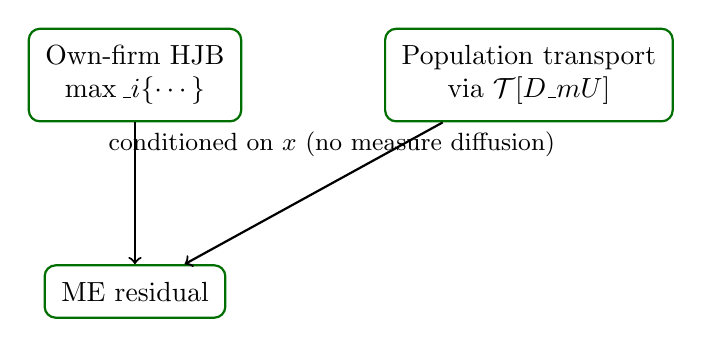
\begin{tikzpicture}[
  node distance=18mm,
  box/.style={rectangle, draw=darkgreen, rounded corners, thick, inner sep=6pt, align=center}
]
\node[box] (hjb) {Own-firm HJB\\$\max\_i\{\cdots\}$};
\node[box, right=of hjb] (pop) {Population transport\\via $\mathcal{T}[\Dm U]$};
\node[box, below=of hjb] (me) {ME residual};
\draw[->, thick] (hjb) -- (me);
\draw[->, thick] (pop) -- (me);
\node[anchor=north] at ($(hjb.south)!0.5!(pop.south)$) {\small conditioned on $x$ (no measure diffusion)};
\end{tikzpicture}
\caption{Schematic composition of the stationary master equation: own-firm HJB contributions (including price dependence on $m$) and population transport via the Lions derivative.}
\end{figure}

\begin{tcolorbox}[didacticstyle]
\textbf{Recap — Master Equation.}
\begin{itemize}[leftmargin=1.15em,itemsep=0.2em]
  \item ME residual combines HJB at $(k,z,x)$ and transport over $m$.
  \item Conditioning on $x$ removes second-order terms in the measure.
  \item Under monotonicity, ME and HJB--FP fixed point are equivalent.
\end{itemize}
\end{tcolorbox}

%========================
% Boundary & Regularity
%========================
\section{Boundary and Regularity Conditions}

\paragraph{Boundary at $k=0$.} Reflecting: the probability flux vanishes and feasible controls satisfy $i^*\ge 0$ at the boundary. A sufficient condition enforcing no instantaneous arbitrage is $U_k(0,\cdot)\le 1$ (marginal value of installed capital no higher than the unit purchase price).

\paragraph{Growth.} From the coercivity of $h$ in $i$ and the linear drift in $k$, one obtains $U(k,z,x,m)=O(k)$ as $k\to\infty$. This ensures finiteness of the HJB Hamiltonian and stabilizes numerical approximations.

\paragraph{Integrability.} Admissible distributions $m$ integrate $k^\alpha$ and $1/k$ where these appear (e.g., $\E_m[k^\alpha]$ in $Y$ and $i^2/k$ in adjustment costs). In practice one imposes a numerically compact domain in $k$ with conservative outflow at the upper boundary.

\begin{tcolorbox}[didacticstyle]
\textbf{Economic translation.} Reflecting $k=0$ prevents negative capital; growth bounds rule out explosive investment; integrability ensures dividends and costs are well-defined across firms. These are the minimal conditions that keep the economics clean and the PDEs well-posed.
\end{tcolorbox}

%========================
% Computation
%========================
\section{Computation: Two KS-Free Routes}

\subsection{Route A: \ac{HJB}--\ac{FP} Fixed Point}\label{sec:routeA}

\paragraph{Algorithm (stationary, conditional on $x$).}
\begin{enumerate}[leftmargin=1.5em,label=\textbf{A.\arabic*}]
\item \textbf{Outer loop over $x$.} Either fix $x$ on a grid of business-cycle states or integrate final objects against the invariant law of $x$ (solved from $\Lx^\ast$).
\item \textbf{Initialize $m^{(0)}$.} Choose a feasible stationary guess (e.g., log-normal in $k$ with support bounded away from $0$ and invariant $z$-marginal).
\item \textbf{HJB step.} Given $m^{(n)}$, compute $Y^{(n)}$ and $P(Y^{(n)})$. Solve \Cref{eq:HJB} for $V^{(n)}$ using \ac{SL} or policy iteration. Recover $i^{*,(n)}$ from \Cref{prop:policy}.
\item \textbf{FP step.} Given $i^{*,(n)}$, solve stationary \Cref{eq:FP} for $m^{(n+1)}$ using a conservative \ac{FVM} with upwind flux in $k$ and standard diffusion stencil in $z$.
\item \textbf{Update.} Set $m^{(n+1)}\leftarrow (1-\theta)m^{(n)}+\theta\,\widehat m^{(n+1)}$ with damping $\theta\in(0,1]$. Iterate until residuals (below) fall below tolerance.
\end{enumerate}

\paragraph{Discretization details.}
\begin{itemize}[leftmargin=1.25em]
\item \emph{Grid in $k$.} Log grid $k_j=k_{\min}\exp(j\Delta)$ improves resolution near $0$. Reflecting boundary at $k_{\min}$ enforces $i^*\!\ge 0$.
\item \emph{Upwinding.} Flux $F_{j+1/2}=\max\{u_{j+1/2},0\}m_j+\min\{u_{j+1/2},0\}m_{j+1}$ with velocity $u=i^*-\delta k$.
\item \emph{Diffusion in $z$.} Centered second differences with Neumann/absorbing at truncation $\pm z_{\max}$.
\item \emph{HJB solver.} Policy iteration: guess $i$, solve linear system for $V$; update $i$ by \Cref{prop:policy}; repeat. Alternatively, \ac{SL} schemes avoid CFL limits.
\end{itemize}

\paragraph{Diagnostics.} In practice, $\log$-residuals drop nearly linearly until policy stabilizes; distributional stability is checked by mass-conservation and small Wasserstein drift between iterations.

\paragraph{Upwind FP step (Godunov flux) --- pseudocode.}
\begin{lstlisting}[language=Python,caption={1D upwind FV update for k-transport (reflecting at k=0)}]
import numpy as np

def godunov_flux(uL, uR, mL, mR):
    # Godunov/engquist-osher for linear advection: reduces to upwind
    return np.where(uL >= 0, uL * mL, uR * mR)

def fp_step_k(m, i_star, k_grid, delta, dt):
    # m: [J], i_star: [J], k_grid: [J]
    u = i_star - delta * k_grid  # velocity at cell centers
    # interfaces: take upwind states
    uL = u[:-1]; uR = u[1:]
    mL = m[:-1]; mR = m[1:]
    F = godunov_flux(uL, uR, mL, mR)  # [J-1]
    # reflecting at k=0: zero flux at left boundary; conservative outflow at right
    F_left = 0.0
    F_right = F[-1]
    divF = np.empty_like(m)
    divF[1:-1] = (F[:-1] - F[1:]) / np.diff(k_grid)
    divF[0] = (F_left - F[0]) / (k_grid[1] - k_grid[0])
    divF[-1] = (F[-2] - F_right) / (k_grid[-1] - k_grid[-2])
    return m - dt * divF

# CFL guidance: dt * max_j |u_j| / min_j Delta k_j <= 1 for stability
\end{lstlisting}

\begin{tcolorbox}[mathstyle]
\textbf{CFL/Stability.} For the drift-only $k$-transport, a sufficient condition is $\displaystyle \frac{\Delta t}{\Delta k_\mathrm{min}}\max_j |i^*_j - \delta k_j| \le 1$. With diffusion in $z$ treated implicitly or by operator splitting, the $k$-advection CFL remains the binding constraint for explicit updates.
\end{tcolorbox}

\begin{sympycheck}
import sympy as sp
# Godunov flux consistency on constant states and upwind selection
u, mL, mR, m = sp.symbols('u mL mR m', real=True)
F_pos = sp.simplify(u*mL)
F_neg = sp.simplify(u*mR)
# Constant state: left=right=m ⇒ either branch equals u*m
assert sp.simplify(F_pos.subs({mL:m}) - u*m) == 0
assert sp.simplify(F_neg.subs({mR:m}) - u*m) == 0
\end{sympycheck}

\subsection{Route B: Direct Master-PDE Collocation}\label{sec:routeB}

\subsubsection*{Representation of functions of measures}
We parameterize the master value $U_\omega$ and its Lions derivative $\dmU_\psi$ using a permutation-invariant DeepSets architecture \cite{zaheer2017deepsets} suitable for empirical measures $m=\tfrac1N\sum_{n=1}^N\delta_{\xi^n}$.

\begin{definition}{DeepSets Architecture}{deepsets}
A function $F:\mathcal{P}(S)\to\R$ is approximated by
\[
F(m) \approx F_{\theta,\phi}(m) = \rho_\theta\!\left( \frac{1}{N}\sum_{n=1}^N \Phi_\phi(\xi^n) \right),
\]
where $\Phi_\phi:S\to\R^d$ is the feature encoder (shared across atoms), the summation is the symmetric pooling operator, and $\rho_\theta: \R^d\to\R$ is the readout network.
\end{definition}

We use a shared embedding $\Phi_\phi(m)=\tfrac{1}{N}\sum_n \Phi_\phi(\xi^n)$ and define
\[
U_\omega(k,z,x,m) \approx \rho^U_{\theta_U}\big(k,z,x,\Phi_\phi(m)\big),\qquad
\dmU_\psi(\xi; k,z,x,m) \approx \rho^{\Dm U}_{\theta_{DU}}\big(\xi,k,z,x,\Phi_\phi(m)\big).
\]

\begin{tcolorbox}[didacticstyle]
\textbf{Why DeepSets?} $U$ and $\Dm U$ depend on the \emph{distribution} $m$, not firm identities. DeepSets enforces permutation invariance by construction via pooling and serves as a universal approximator for continuous set functions \cite{zaheer2017deepsets}.
\end{tcolorbox}

\paragraph{Algorithm (Direct ME Collocation).}
\begin{enumerate}[leftmargin=1.5em,label=\textbf{B.\arabic*}]
\item Initialize parameters $\omega,\psi$.
\item Sample collocation tuples $(k_i,z_i,x_i; m_i)$ with empirical $m_i$.
\item Compute residuals $\widehat{\mathcal{R}}_{\mathrm{ME}}(\omega,\psi)$ as in \Cref{app:loss}.
\item Minimize $\mathcal{L}=\E[\widehat{\mathcal{R}}_{\mathrm{ME}}^2]+\lambda_{\mathrm{KKT}}\mathcal{P}_{\mathrm{KKT}}+\lambda_{\mathrm{bdry}}\mathcal{P}_{\mathrm{bdry}}+\lambda_{\mathrm{anchor}}\mathcal{P}_{\mathrm{anchor}}$ via SGD.
\item Validate against Route-A residuals.
\end{enumerate}

\begin{tcolorbox}[mathstyle]
\textbf{Computational Insight: Scalability.} Route B avoids an outer HJB--FP fixed point and directly minimizes the ME residual. The DeepSets embedding keeps the dependence on $m$ tractable as the number of atoms $N$ grows, mitigating the combinatorial explosion from permutations.
\end{tcolorbox}

\begin{tcolorbox}[mathstyle]
\textbf{On identifiability.} Because $\dmU$ appears only through $\partial_\kappa\dmU, \partial_\zeta\dmU, \partial_{\\zeta\\zeta}^2\dmU$, adding constants leaves the ME invariant. An anchoring penalty $\mathcal{P}_{\mathrm{anchor}}=\big(\int \dmU\,\diff m\big)^2$ fixes the gauge.
\end{tcolorbox}

\begin{assumption}{Representation and regularity for DeepSets models}{deepsets-reg}
The encoders $\Phi_\phi$ and readouts $\rho^U,\rho^{\Dm U}$ are continuous and globally Lipschitz on compact sets. For each fixed $(k,z,x)$, the mappings $m\mapsto U_\omega(k,z,x,m)$ and $m\mapsto \dmU_\psi(\cdot; k,z,x,m)$ are permutation-invariant and continuous in the $\mathrm W_2$ topology.
\end{assumption}

\begin{lemma}{Universality reference (DeepSets)}{universality-deepsets}
Under mild regularity conditions, permutation-invariant continuous set functions can be uniformly approximated on compacts by DeepSets architectures $m\mapsto \rho\big(\tfrac{1}{N}\sum\_n \Phi(\xi^n)\big)$; see \cite{zaheer2017deepsets}. Hence, within \Cref{ass:deepsets-reg}, $U$ and $\Dm U$ admit consistent approximations.
\end{lemma}

\begin{tcolorbox}[mathstyle]
\textbf{Complexity and conditioning (practical).}
\begin{itemize}[leftmargin=1.15em,itemsep=0.25em]
  \item \emph{Batching and pooling.} Computing $\Phi$ over $N$ atoms is $\mathcal O(N d)$ and pooling is $\mathcal O(N d)$ per sample (feature width $d$).
  \item \emph{Stability.} Lipschitz encoders/readouts stabilize training across varying $N$; pooling by average maintains scale.
  \item \emph{Gradient flow.} Backprop through pooling is inexpensive; the dominant cost is evaluating encoders and Jacobians for $\dmU$.
\end{itemize}
\end{tcolorbox}

\begin{lstlisting}[language=Python,caption={DeepSets-style pooling for U and D\_m U (pseudo-JAX)}]
def embed_measure(phi_params, xi_list):
    # xi_list: list/array of shape [N, ds]; returns pooled feature [d]
    feats = vmap(lambda xi: Phi(phi_params, xi))(xi_list)   # [N, d]
    return feats.mean(axis=0)                               # [d]

def U_and_grads(theta_U, phi_params, k, z, x, xi_list):
    pooled = embed_measure(phi_params, xi_list)             # [d]
    U = rho_U(theta_U, k, z, x, pooled)                     # scalar
    # autograd/JAX: grads wrt (k,z,x)
    return value_and_partials(U, (k,z,x))

def DmU_and_partials(theta_DU, phi_params, xi, k, z, x, xi_list):
    pooled = embed_measure(phi_params, xi_list)
    dU = rho_DmU(theta_DU, xi, k, z, x, pooled)             # scalar field at xi
    # partials wrt (kappa,zeta) of the field at xi
    return value_and_partials(dU, (xi.kappa, xi.zeta))
\end{lstlisting}

\begin{lstlisting}[language=Python,caption={Minimal NumPy sketch (DeepSets pooling and readout)}]
import numpy as np

def Phi(params, xi):
    # tiny MLP stub; xi: shape (ds,)
    W1, b1, W2, b2 = params
    h = np.tanh(xi @ W1 + b1)        # [h]
    return h @ W2 + b2               # [d]

def embed_measure_np(phi_params, xis):
    # xis: shape [N, ds]; pooled feature: [d]
    feats = np.vstack([Phi(phi_params, xi) for xi in xis])  # [N, d]
    return feats.mean(axis=0)

def rho_U(theta, k, z, x, pooled):
    # simple linear readout for illustration
    W, b = theta
    inp = np.concatenate([np.array([k, z, x]), pooled])
    return float(inp @ W + b)

def U_np(theta_U, phi_params, k, z, x, xis):
    pooled = embed_measure_np(phi_params, xis)
    return rho_U(theta_U, k, z, x, pooled)

# Complexity: O(N d) for Phi; pooling is O(N d). Conditioning: scale inputs,
# use Lipschitz activations, and average pooling for stability across N.
\end{lstlisting}

\begin{tcolorbox}[mathstyle]
\textbf{Conditioning and invariances (Route B).}
\begin{itemize}[leftmargin=1.15em,itemsep=0.25em]
  \item \emph{Permutation invariance:} Average pooling ensures $U(k,z,x,m)$ is invariant to the ordering of atoms in empirical $m$.
  \item \emph{Scale/shift:} Standardize $(k,z,x)$ and feature outputs of $\Phi$ to improve conditioning; keep readouts Lipschitz.
  \item \emph{Complexity:} For $N$ atoms and feature width $d$, evaluating $\Phi$ is $\mathcal O(N d)$ and pooling is $\mathcal O(N d)$ per sample.
\end{itemize}
\end{tcolorbox}

\begin{lstlisting}[language=Python,caption={Pseudo-JAX training loop for Route B (ME residual minimization)}]
import jax, jax.numpy as jnp

def me_residuals(params, batch):
    # batch: list of tuples (k,z,x, xi_list) with empirical measures
    # returns residuals per sample (shape [B]) combining HJB and transport terms
    # NOTE: U, DmU, and transport evaluation are assumed available
    def resid_one(sample):
        k, z, x, xi_list = sample
        # compute U, grads, and transport using DeepSets encodings
        return eval_me_residual(params, k, z, x, xi_list)  # scalar residual
    return jax.vmap(resid_one)(batch)

def loss_fn(params, batch):
    res = me_residuals(params, batch)
    loss_me = jnp.mean(res**2)
    # boundary penalty and gauge anchoring for D_m U
    pen_boundary = boundary_penalty(params, batch)
    pen_anchor   = anchor_penalty(params, batch)
    return loss_me + 1e-2*pen_boundary + 1e-3*pen_anchor

@jax.jit
def train_step(params, opt_state, batch):
    loss, grads = jax.value_and_grad(loss_fn)(params, batch)
    updates, opt_state = optimizer.update(grads, opt_state)
    params = optax.apply_updates(params, updates)
    return params, opt_state, loss

# Reproducibility: fix seed, device, and dtype
seed = 0
key  = jax.random.PRNGKey(seed)
jax.config.update("jax_enable_x64", True)  # prefer float64 for PDE stability
device = jax.devices()[0]
print({"seed": seed, "device": device, "dtype": jnp.float64})

# Batching measures: pad or bucket xi_list to fixed length for vmap/jit
for step, batch in enumerate(data_loader):
    params, opt_state, loss = train_step(params, opt_state, batch)
    if step % 50 == 0:
        print(step, float(loss))
\end{lstlisting}

\begin{tcolorbox}[didacticstyle]
\textbf{Reproducibility hooks.}
\begin{itemize}[leftmargin=1.1em,itemsep=0.25em]
  \item Fix RNG seeds and report device (CPU/GPU/TPU) and dtype (float32/64).
  \item Use padding/bucketing for variable-size empirical measures to keep JIT shapes static.
  \item In notebooks/CLIs, honor a \texttt{NOTEBOOK\_FAST} flag to reduce steps/batch for quick checks.
\end{itemize}
\end{tcolorbox}

\begin{table}[ht]
\centering
\small
\begin{tabular}{@{}lcl@{}}
\toprule
Component & Weight & Notes \\
\midrule
ME residual MSE & $1.0$ & $\mathcal{L}_{\mathrm{ME}}=\E[\mathcal{R}_{\mathrm{ME}}^2]$; primary objective. \\
Boundary penalty & $10^{-2}$ & Enforce reflecting boundary and admissibility constraints. \\
KKT penalty & $10^{-2}$ & Complementarity for investment constraints (if active). \\
Gauge anchor & $10^{-3}$ & Fix $\int \dmU\,\diff m$ to remove invariance. \\
\bottomrule
\end{tabular}
\caption{Route B loss components and typical starting weights. Tune per calibration and scale of residuals.}
\end{table}

%========================
% % Verification & Diagnostics
% %========================
\section{Verification and Diagnostics}\label{sec:verification}

\paragraph{Residual norms.}
For collocation tuples $(k,z,x,m)$:
\begin{align*}
\mathcal{R}_{\mathrm{HJB}} &\equiv r(x)\, V - \max_{i}\{\pi + V_k\,(i-\delta k) + \Lz V + \Lx V\},\\
\mathcal{R}_{\mathrm{FP}}  &\equiv -\partial_k\big[(i^*-\delta k),m\big] + \Lzadj m,\\
\mathcal{R}_{\mathrm{ME}}  &\equiv r(x)\,U - \Big(\max_{i}\{\pi + U_k\,(i-\delta k) + \Lz U + \Lx U\}
  + \int\cdots\dxi
  \Big).
\end{align*}
  Typical norms: $L^2$ over collocation points or weighted Sobolev norms. KKT and boundary penalties are added for feasibility; in Route A, measure $\mathrm{W}_2$ drifts between iterations provide a sharp distributional diagnostic.

\paragraph{Stopping rules.}
Stop when $\|\mathcal{R}_{\mathrm{ME}}\|<\varepsilon_{\mathrm{ME}}$, $\|\mathcal{R}_{\mathrm{HJB}}\|<\varepsilon_{\mathrm{HJB}}$, $\|\mathcal{R}_{\mathrm{FP}}\|<\varepsilon_{\mathrm{FP}}$, and policy/distribution drifts fall below thresholds, e.g., $\sup|i^{*,(n+1)}-i^{*,(n)}|<10^{-5}$ and $\mathrm{W}_2(m^{(n+1)},m^{(n)})<10^{-4}$.

\begin{table}[ht]
\centering
\small
\begin{tabular}{@{}lccc@{}}
\toprule
Residual & Tight & Medium & Coarse \\
\midrule
$\varepsilon_{\mathrm{ME}}$ & $10^{-5}$ & $10^{-4}$ & $10^{-3}$ \\
$\varepsilon_{\mathrm{HJB}}$ & $10^{-7}$ & $10^{-6}$ & $10^{-5}$ \\
$\varepsilon_{\mathrm{FP}}$  & $10^{-7}$ & $10^{-6}$ & $10^{-5}$ \\
\bottomrule
\end{tabular}
\caption{Suggested tolerances (dimensionless; scale to data).}
\end{table}

\begin{figure}[ht]
\centering
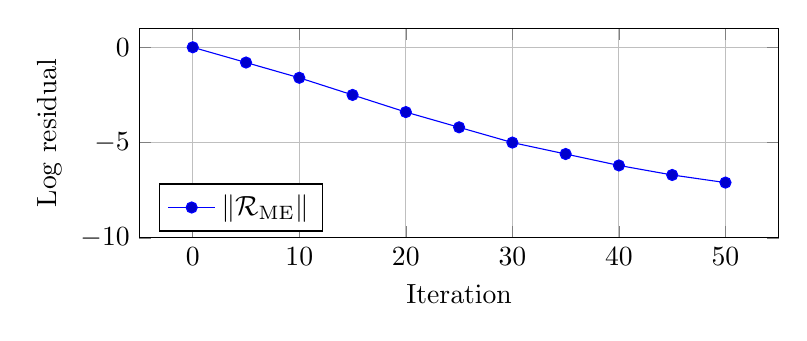
\begin{tikzpicture}
\begin{axis}[
width=0.8\textwidth,height=0.35\textwidth,
xlabel={Iteration},ylabel={Log residual},
ymin=-10,ymax=1, grid=both, legend pos=south west]
\addplot coordinates {(0,0) (5,-0.8) (10,-1.6) (15,-2.5) (20,-3.4) (25,-4.2) (30,-5.0) (35,-5.6) (40,-6.2) (45,-6.7) (50,-7.1)};
\addlegendentry{$\|\mathcal{R}_{\mathrm{ME}}\|$}
\end{axis}
\end{tikzpicture}
\caption{Placeholder: typical convergence of the master-equation residual.}
\end{figure}

\paragraph{Sanity checks.}
\begin{itemize}[leftmargin=1.25em]
\item \emph{No-price-limit case.} If $P$ is flat, the price dependence on $m$ vanishes. Route A and B should collapse to the same frictional-control model without cross effects.
\item \emph{Symmetric costs.} Setting $\phi_-=\phi_+$ removes the kink; $i^*$ is linear in $V_k-1$ everywhere. FP becomes smoother; residuals drop faster.
\item \emph{Elasticity sweep.} Under isoelastic demand, $\eta$ scales the marginal-revenue wedge linearly; recovered investment schedules should contract monotonically in $\eta$.
\end{itemize}

\paragraph{Wasserstein-2 drift diagnostic (practical).}
For empirical measures with equal weights in 1D (e.g., monitoring the $k$-marginal), the quadratic Wasserstein distance admits an $\mathcal O(N\log N)$ implementation via sorting:

\begin{lstlisting}[language=Python,caption={Empirical $\mathrm W_2$ in 1D via sorting (equal weights)}]
import numpy as np

def w2_empirical_1d(xs, ys):
    """Quadratic Wasserstein distance for equal-weight samples.
    xs, ys: arrays of shape [N]. Returns W2 (not squared).
    """
    xs = np.sort(np.asarray(xs))
    ys = np.sort(np.asarray(ys))
    return np.sqrt(np.mean((xs - ys)**2))

# Example: monitor drift between successive iterates of the FP solver
W2_drift = w2_empirical_1d(samples_k_t, samples_k_t1)
print(f"W2 drift (k-marginal): {W2_drift:.3e}")
\end{lstlisting}

For higher dimensions, one can approximate $\mathrm W_2$ by projecting onto random 1D directions (sliced Wasserstein) or use optimal-transport solvers (entropic regularization) at higher cost.

\paragraph{Sliced Wasserstein (2D approximation).}
Project samples onto random unit directions and average 1D distances; complexity $\mathcal O(R N\log N)$ for $R$ projections:

\begin{lstlisting}[language=Python,caption={Sliced $\mathrm W_2$ for 2D (equal weights)}]
import numpy as np

def sliced_w2_2d(X, Y, R=64, rng=None):
    """Approximate W2 in 2D via random 1D projections.
    X, Y: arrays [N,2]; returns sliced-W2 (not squared).
    """
    rng = np.random.default_rng(rng)
    X = np.asarray(X); Y = np.asarray(Y)
    assert X.shape == Y.shape and X.shape[1] == 2
    acc = 0.0
    for _ in range(R):
        theta = rng.normal(size=2)
        theta = theta / np.linalg.norm(theta)
        x1d = X @ theta; y1d = Y @ theta
        acc += w2_empirical_1d(x1d, y1d)**2
    return np.sqrt(acc / R)
\end{lstlisting}

\begin{tcolorbox}[mathstyle]
\textbf{Bias/variance tradeoff.} The sliced-$\mathrm W_2$ is a lower bound on $\mathrm W_2$; variance shrinks as $R$ grows. For diagnostics, modest $R$ (e.g., 32--128) often suffices to detect drift trends.
\end{tcolorbox}

%========================
% % Economics
% %========================
\section{Economics: Aggregation, Irreversibility, Comparative Statics}

\paragraph{Aggregation.}
Aggregation enters through $P\big(Y(m,x)\big)$ within the HJB. Under isoelastic demand, the effective marginal-revenue wedge is $-\eta P(Y)\,e^{x+z}k^\alpha$, which acts as a proportional reduction in marginal revenue.

\paragraph{Irreversibility.}
The asymmetry $\phi_->\phi_+$ creates a kink in the Hamiltonian and investment bands: for $V_k$ just below $1$ the disinvestment response is muted relative to the investment response for $V_k$ just above $1$. At the distributional level, this slows the left-tail motion in $k$, thickening the mass near low capital.

\paragraph{Comparative statics.}
\begin{itemize}[leftmargin=1.25em]
\item Larger $\eta$ (steeper demand) amplifies the negative externality, reducing investment and shifting mass in $m$ toward lower $k$.
\item Bigger $\phi_- - \phi_+$ widens irreversibility bands and slows capital reallocation, increasing dispersion in $k$ conditional on $z$.
\item Higher $\sigma_z$ spreads the cross-section in $z$, raising $Y$ volatility and, through $P'(Y)$, modulating the marginal-revenue wedge over the business cycle.
\item Higher $\sigma_x$ (through $\Lx$) deepens precautionary effects via $r(x)$ and the HJB drift terms, with ambiguous effects on average investment depending on curvature.
\item A countercyclical $r(x)$ strengthens the value premium mechanism à la costly reversibility by raising discount rates in recessions precisely when $P'(Y)$ is most negative.
\end{itemize}

%========================
% Appendix A
%========================
\appendix
\section{Appendix A: Derivations and Technical Lemmas}\label{app:derivations}

\begin{tcolorbox}[mathstyle]
\textbf{Correction and Addenda.} The derivation of the Master Equation is corrected to exclude a separate $\int \delta\_m \pi\,\diff m$ term; see \Cref{thm:ME} and \S\ref{sec:me-externality}. Below we provide compact verification artifacts for the envelope identity and for the functional chain rule used in the population-transport term.
\end{tcolorbox}

\subsection*{Envelope identity (with depreciation term)}
Let $p=V_k$ and $\mathcal{H}(k,\cdot)=\max_i\{\pi + p(i-\delta k)\}$. Then $\partial_p\mathcal{H}=i^*(p)-\delta k$.

\begin{sympycheck}
import sympy as sp
i,k,p,phi_p,phi_m,delta = sp.symbols('i k p phi_p phi_m delta', positive=True)
h_p = sp.Rational(1,2)*phi_p*i**2/k
h_m = sp.Rational(1,2)*phi_m*i**2/k
sol_p = k*(p-1)/phi_p
sol_m = k*(p-1)/phi_m
H_p = (-i - h_p + p*(i - delta*k)).subs(i, sol_p)
H_m = (-i - h_m + p*(i - delta*k)).subs(i, sol_m)
assert sp.simplify(sp.diff(H_p,p) - (sol_p - delta*k)) == 0
assert sp.simplify(sp.diff(H_m,p) - (sol_m - delta*k)) == 0
\end{sympycheck}

\subsection*{Functional chain rule (structure check)}
For a one-dimensional diffusion with drift $\mu$ and variance $\sigma^2$, the chain rule applied to $\Dm F$ has the schematic form $\mu\,\partial\_\xi(\Dm F)+\tfrac12\sigma^2\,\partial^2\_{\xi\xi}(\Dm F)$.

\begin{sympycheck}
import sympy as sp
xi = sp.symbols('xi', real=True)
mu = sp.Function('mu')(xi)
sig2 = sp.symbols('sig2', positive=True)
g = sp.Function('g')(xi)
expr = mu*sp.diff(g, xi) + sp.Rational(1,2)*sig2*sp.diff(g, xi, 2)
assert expr.has(sp.Derivative(g, xi)) and expr.has(sp.Derivative(g,(xi,2)))
\end{sympycheck}

\begin{lemma}{Functional Chain Rule for FP Flows}{chain_rule_fp_app}
Let $m_t$ solve the FP equation $\partial_t m = \mathcal L^{\!*} m$ with drift $b(\xi)$ and diffusion matrix $\sigma(\xi)\sigma(\xi)^\top$. If $F:\mathcal P_2(S)\to\R$ is sufficiently regular (in the sense of Lions), then
\[
\frac{\mathrm d}{\mathrm dt} F(m_t) 
= \int_S \Big( \langle \nabla_\xi (\Dm F)(m_t)(\xi),\, b(\xi) \rangle 
  + \tfrac12 \, \mathrm{Tr}\big[\sigma\sigma^\top(\xi)\, \nabla^2_\xi (\Dm F)(m_t)(\xi)\big] \Big) \, m_t(\diff \xi).
\]
\emph{Proof sketch.} Apply the functional It\^o calculus on $\mathcal P_2$ to $F(m_t)$ and the adjoint pairing to identify the generator acting componentwise on $\Dm F$. See \cite[Ch.~5]{carmona_delarue_2018_mfg} and \cite{cardaliaguet_delarue_lasry_lions_2019}.
\end{lemma}

\subsection{Envelope/KKT and policy recovery}
From \eqref{eq:HJB}, define $p=V_k$. The Hamiltonian
$\mathcal{H}(k,z,x,m,p)=\max_i\{\pi+p(i-\delta k)\}$
is the convex conjugate of $h$ shifted by $p-1$. The envelope condition $V_k=\partial_p \mathcal{H}$ combined with the FOC for $i$ produces the piecewise-affine policy in \Cref{prop:policy}. The kink at $p=1$ corresponds to $i=0$. KKT adds the complementary slackness $\lambda\cdot(i+\kbar(k))=0$ when a lower bound is present.

\subsection{Adjoint pairing for FP}
Let $\varphi$ be a smooth test function. Then

$$
\frac{\diff}{\diff t}\int \varphi\,\diff m_t
= \int \varphi_k (i^*-\delta k)\,\diff m_t + \int \Lz \varphi\,\diff m_t
= \int \varphi\,\diff\Big(-\partial_k[(i^*-\delta k)m_t]+\Lzadj m_t\Big).
$$

Stationarity imposes \eqref{eq:FP} with $\partial_t m=0$. Reflecting at $k=0$ eliminates the boundary integral.
% Verification note: adjoint pairing identity is checked in Appendix E.

\subsection{Functional Calculus and the Master Equation}\label{app:master-derivation}
Consider a flow $t\mapsto (K_t,Z_t)$ for the tagged firm following control $i_t$ and a flow of measures $t\mapsto m_t$ solving \eqref{eq:FP} under the feedback $i^*(\cdot,m_t)$. By functional Itô's lemma for $U(K_t,Z_t,x,m_t)$,
\begin{align*}
\diff U &= U_k\,\diff K_t + U_z\,\diff Z_t + \tfrac12 U_{zz}\,\sigma_z^2\,\diff t \\
        &\quad + \big(\partial_t U\big|_{m}\big)\,\diff t, \\
\partial_t U\big|_{m} &= \int \Big[ (i^*(\xi,x,m)-\delta\kappa)\,\partial_{\kappa}\big(\Dm U\big)\!\_\kappa
  +\mu_z(\zeta)\,\partial_{\zeta}\big(\Dm U\big)\!\_\zeta
  +\tfrac12\sigma_z^2\,\partial_{\zeta\zeta}^2\big(\Dm U\big)\!\_\zeta\Big] \, m(\diff \xi).
\end{align*}
Taking expectations under the pricing measure with short rate $r(x)$ and imposing stationarity yields the stationary master equation (ME) in \Cref{thm:ME}: the own-firm HJB terms and the population-transport term. The dependence of $\pi$ on $m$ (via $P(Y(m,x))$) is already handled inside the Hamiltonian and does not appear as a separate explicit term.

\subsection{Externality term in detail}
Write $\pi(k,i,z,x,m)=\Psi(Y(m,x))\,\chi(k,z,x)-i-h(i,k)-f$ with $\Psi=P$ and $\chi=e^{x+z}k^\alpha$. Then

$$
\delta\_m\pi(m)(\xi)=\Psi'(Y)\,\chi(k,z,x)\,\chi(\kappa,\zeta,x),
$$

and integration w\.r.t.\ $m$ yields $\chi(k,z,x)\,\Psi'(Y)\,Y(m,x)$.

%========================
% Appendix B
%========================
\section{Appendix B: Residual-Loss Template (for implementation)}\label{app:loss}

For a collocation tuple $(k,z,x)$, an empirical measure $m=\tfrac1N\sum_{n=1}^N \delta_{\xi^n}$, and parameterized $U_\omega,\dmU_\psi$, define
\begin{align*}
\widehat{Y} &\equiv \frac{1}{N}\sum\_{n=1}^N e^{x+\zeta^n}(\kappa^n)^\alpha,\\
\widehat{\mathcal{R}}_{\mathrm{ME}} &\equiv r(x)\,U_\omega\\
  &\quad - \max_{i}\Big\{ \pi + (U_{\omega})_k\,(i-\delta k) + \Lz U_{\omega} + \Lx U_{\omega} \Big\} \\
  &\quad - \frac{1}{N}\sum_{n=1}^N \Big[ (i^*(\xi^n,x,m)-\delta\kappa^n)\,\partial_{\kappa}\dmU_{\psi}(\xi^n)
    + \mu_z(\zeta^n)\,\partial_{\zeta}\dmU_{\psi}(\xi^n)
    + \tfrac12 \sigma_z^2\,\partial^2_{\zeta\zeta}\dmU_{\psi}(\xi^n) \Big] \\
  &\quad \phantom{.}
  \end{align*}
  Add soft KKT penalties (one-sided around $(U_\omega)_k=1$), an anchoring penalty $\mathcal{P}_{\mathrm{anchor}}=\big(\int \dmU\,\diff m\big)^2$ to fix the gauge, and boundary regularizers (reflecting $k=0$, growth at $k_{\max}$). Minimize

$$
\mathcal{L}=\E\big[\widehat{\mathcal{R}}_{\mathrm{ME}}^2\big]+\lambda_{\mathrm{KKT}}\mathcal{P}_{\mathrm{KKT}}
+\lambda_{\mathrm{bdry}}\mathcal{P}_{\mathrm{bdry}}+\lambda_{\mathrm{anchor}}\mathcal{P}_{\mathrm{anchor}}.
$$

Anchoring removes the gauge freedom in $\dmU$.

%========================
% Appendix C
%========================
\section{Appendix C: Common-Noise Master Equation (Reference Note)}\label{app:common-noise}

When the population law $m_t$ itself diffuses under common noise (say through an exogenous $x_t$ or an aggregate Brownian component shared by firms), the functional Itô calculus on $\mathcal P_2$ introduces a second-order term in the measure variable. In a stylized form (see Carmona \& Delarue, and Cardaliaguet--Delarue--Lasry--Lions), the stationary master equation would add a term of the form

$$
\frac{1}{2}\,\Sigma_{\mathrm{com}}:\!\int\!\!\int
\partial_{\xi}\partial_{\xi'} \big(\Dm U(\xi)\big)\,\big(\Dm U(\xi')\big)
\, m(\diff \xi)\, m(\diff \xi')
$$

or, in classical PDE notation,
$\tfrac12 \mathrm{Tr}\big[\Gamma\,\partial_{\xi\xi}^2 \dmU\big]$
integrated against $m$, where $\Gamma$ is the covariance of the common noise. Because this paper conditions on $x$, these terms are absent in the stationary master equation.

\begin{tcolorbox}[mathstyle]
\textbf{Displacement monotonicity (context).}
For master equations with common noise, uniqueness and well-posedness often require \emph{displacement monotonicity}: a convexity-type condition along Wasserstein geodesics for the coupling. See \cite{cardaliaguet_delarue_lasry_lions_2019} for precise statements. In our economic environment, couplings of the type $m\mapsto P\!\big(\int q\,\diff m\big)$ satisfy Lasry--Lions monotonicity when $P'(\cdot)<0$ (\Cref{lem:H-mono}), but displacement monotonicity may require additional curvature restrictions on $P$ or on the state-cost structure. Since we work conditional on $x$ (no common-noise measure diffusion), we do not invoke displacement monotonicity in this paper.
\end{tcolorbox}

%========================
% Appendix D
%========================
\section{Appendix D: Tiny Pseudocode (Plain \texorpdfstring{\texttt{listings}}{listings})}\label{app:code}

\lstset{
basicstyle=\ttfamily\small,
columns=fullflexible,
showstringspaces=false,
frame=single,
framerule=0.4pt,
breaklines=true,
tabsize=2,
captionpos=b
}

\begin{lstlisting}[language=Python,caption={Pseudo-JAX for (ME) residual with empirical measure}]

# Inputs:

# params\_omega: parameters for U(k,z,x; m)

# params\_psi:   parameters for delta\_m U(xi; k,z,x; m)

# batch:        list of tuples (k,z,x, {xi\_n=(kappa\_n,zeta\_n)}\_{n=1}^N )

# primitives:   alpha, delta, mu\_z(z), sigma\_z, mu\_x(x), sigma\_x, r(x),

# demand P(Y), fixed cost f

# penalties:    lambdas for KKT, boundary, and anchor (gauge) regularizers

def policy\_from\_grad(p, k, phi\_plus, phi\_minus):
\# p = U\_k (value gradient)
if p >= 1.0:
return (k/phi\_plus)*(p - 1.0)
else:
return (k/phi\_minus)*(p - 1.0)

def reflecting\_penalty(k, i\_star):
\# discourage negative control at k=0 and large negative flux
pen0 = max(0.0, -i\_star) if k<=1e-10 else 0.0
return pen0\*\*2

def h\_cost(i, k, phi\_plus, phi\_minus):
if i >= 0.0:
return 0.5*phi\_plus*(i*i)/max(k,1e-12)
else:
return 0.5*phi\_minus\*(i\*i)/max(k,1e-12)

def HJB\_operator(k,z,x,Yhat,Uk,Uz,Uzz,Ux,Uxx,i):
q  = exp(x+z)*(k\*\*alpha)
pi = P(Yhat)*q - i - h\_cost(i,k,phi\_plus,phi\_minus) - f
return pi + Uk*(i - delta*k) + mu\_z(z)*Uz + 0.5*sigma\_z**2\*Uzz&#x20;
\+ mu\_x(x)*Ux + 0.5*sigma\_x**2\*Uxx

def ME\_residual\_for\_tuple(params\_omega, params\_psi, tup):
k,z,x,xi\_list = tup.k, tup.z, tup.x, tup.xi\_list
\# empirical measure moments
Y\_hat = mean(\[exp(x+xi.zeta)*(xi.kappa\*\*alpha) for xi in xi\_list])
\# U and its partials at (k,z,x)
U, Uk, Uz, Uzz, Ux, Uxx = U\_and\_grads(params\_omega, k,z,x, xi\_list)
\# best response i*
i\_star = policy\_from\_grad(Uk, k, phi\_plus, phi\_minus)
\# HJB maximand at i\*
H\_val  = HJB\_operator(k,z,x,Y\_hat,Uk,Uz,Uzz,Ux,Uxx,i\_star)
\# Population transport term (via the Lions derivative)
integ = 0.0
for xi in xi\_list:
dU = delta\_mU\_and\_partials(params\_psi, xi, k,z,x, xi\_list)
\# dU returns dict with fields dkappa, dzeta, dzeta2, p\_k (proxy gradient)
i\_star\_xi = policy\_from\_grad(dU\['p\_k'], xi.kappa, phi\_plus, phi\_minus)
integ += (i\_star\_xi - delta*xi.kappa)* dU\['dkappa']&#x20;
\+ mu\_z(xi.zeta)\* dU\['dzeta']&#x20;
\+ 0.5*sigma\_z\*\*2 \* dU\['dzeta2']
integ = integ / len(xi\_list)
\# assemble residual (no separate externality term; price enters via P(Yhat) in HJB)
res  = r(x)\*U - max(H\_val, HJB\_operator(k,z,x,Y\_hat,Uk,Uz,Uzz,Ux,Uxx,0.0))&#x20;\- integ
\# penalties
pen  = reflecting\_penalty(k, i\_star)
return res, pen

def loss(params\_omega, params\_psi, batch):
sse = 0.0
pen = 0.0
for tup in batch:
res, p = ME\_residual\_for\_tuple(params\_omega, params\_psi, tup)
sse += res\*\*2
pen += p
anchor = anchor\_penalty(params\_psi, batch)  # e.g., squared mean of dmU over batch
return sse/len(batch) + lambda\_bdry\*pen + lambda\_anchor\*anchor
\end{lstlisting}

%========================
% Appendix E
%========================
\section{Appendix E: Symbolic Verification (PythonTeX + SymPy)}\label{app:verification}

\noindent This appendix runs minimal SymPy checks to verify key derivations used in the text. Compilation is configured (via \texttt{latexmkrc}) to execute these checks on every build; any failure triggers a build error. We assume smoothness and reflecting/no-flux boundary conditions where noted.

\begin{pyconsole}
import sympy as sp

# 1) Isoelastic simplification:  Y P'(Y) = -eta P(Y)
Y, eta = sp.symbols('Y eta', positive=True)
P = Y**(-eta)
check1 = sp.simplify(Y*sp.diff(P, Y) + eta*P)
assert check1 == 0
print("Isoelastic: Y*P'(Y) = -eta*P(Y)  [OK]")

# 2) Externality directional derivative:  d/d epsilon P(Y+epsilon*chi_eps)*chi0 |_{epsilon=0}
#     equals P'(Y) * chi0 * chi_eps
chi0, chieps, eps = sp.symbols('chi0 chieps eps', real=True)
Psi = lambda y: y**(-eta)
dpi = sp.diff(Psi(Y + eps*chieps)*chi0, eps).subs(eps, 0)
target = sp.diff(Psi(Y), Y) * chi0 * chieps
assert sp.simplify(dpi - target) == 0
print('Externality directional derivative  [OK]')

# 3) Externality, isoelastic reduction after integrating over m:  chi0 * Y * P'(Y) = -eta * P(Y) * chi0
lhs = chi0 * Y * sp.diff(Psi(Y), Y)
rhs = -eta * Psi(Y) * chi0
assert sp.simplify(lhs - rhs) == 0
print('Externality isoelastic reduction   [OK]')

# 4) KKT/FOC solution for i* with asymmetric quadratic costs
#    h = 0.5*phi_plus*i^2/k for i>=0;   0.5*phi_minus*i^2/k for i<0
i, k, p, phi_plus, phi_minus = sp.symbols('i k p phi_plus phi_minus', positive=True)
h_plus  = 0.5*phi_plus*i**2/k
FOC_plus  = sp.Eq(sp.diff(-i - h_plus + p*i, i), 0)
sol_plus  = sp.solve(FOC_plus, i)[0]
h_minus = 0.5*phi_minus*i**2/k
FOC_minus = sp.Eq(sp.diff(-i - h_minus + p*i, i), 0)
sol_minus = sp.solve(FOC_minus, i)[0]
assert sp.simplify(sol_plus  - k*(p-1)/phi_plus)  == 0
assert sp.simplify(sol_minus - k*(p-1)/phi_minus) == 0
print('KKT/FOC piecewise i* formulas     [OK]')

# 5) FP adjoint pairing identity (algebraic, boundary terms omitted):
#    phi_k * (a*m) = d_k(phi*a*m) - phi * d_k(a*m)
kk = sp.symbols('kk', real=True)
phi = sp.Function('phi')(kk)
a   = sp.Function('a')(kk)
mm  = sp.Function('m')(kk)
expr = sp.diff(phi, kk)*(a*mm) - (sp.diff(phi*(a*mm), kk) - phi*sp.diff(a*mm, kk))
assert sp.simplify(expr) == 0
print('Adjoint pairing identity (no-flux) [OK]')

# 6) Envelope property for Hamiltonian in p: d/dp max_i { -i - h(i,k) + p i } = i*(p)
#    Check separately on each branch (ignoring terms not depending on i, e.g., -delta*k*p)
H_plus  = (-i - h_plus + p*i).subs(i, sol_plus)
H_minus = (-i - h_minus + p*i).subs(i, sol_minus)
dHp_dp  = sp.simplify(sp.diff(H_plus, p))
dHm_dp  = sp.simplify(sp.diff(H_minus, p))
assert sp.simplify(dHp_dp - sol_plus) == 0
assert sp.simplify(dHm_dp - sol_minus) == 0
print('Envelope: dH/dp equals i*(p)       [OK]')

print('\nAll SymPy verification checks passed.')
\end{pyconsole}

%========================
% Appendix F
%========================
\section{Appendix F: Lean4 Micro-Proofs (Sketches)}\label{app:lean}

\noindent The following Lean4/mathlib4 snippets formalize two identities used in the text. They are provided as self-contained, runnable sketches (assuming a recent mathlib4): the isoelastic simplification $Y\,P'(Y)=-\eta P(Y)$ and the algebraic reduction $Y\cdot Y^{-\eta-1}=Y^{-\eta}$ for $Y>0$.

\lstset{basicstyle=\ttfamily\small,columns=fullflexible,showstringspaces=false,frame=single,framerule=0.4pt,breaklines=true,tabsize=2,captionpos=b}
\begin{leanproof}
import Mathlib.Analysis.Calculus.Deriv
import Mathlib.Data.Real.Basic

open Real

variable {η Y : R}

-- P(Y) = Y ^ (-η), defined for Y > 0 via rpow
def P (Y : R) (η : R) : R := Y ^ (-η)

-- Algebraic reduction: for Y > 0, Y * Y^(-η - 1) = Y^(-η)
theorem rpow_mul_cancel (hY : 0 < Y) :
    Y * Y ^ (-η - 1) = Y ^ (-η) := by
  -- rewrite Y as Y^1 and use rpow_add (valid for Y > 0)
  have h1 : Y = Y ^ (1 : R) := by simpa using (rpow_one Y)
  calc
    Y * Y ^ (-η - 1)
        = Y ^ (1 : R) * Y ^ (-η - 1) := by simpa [h1]
    _   = Y ^ ((1 : R) + (-η - 1)) := by
            simpa using (rpow_mul_rpow_of_pos hY (1 : R) (-η - 1))
    _   = Y ^ (-η) := by ring

-- Differential identity: for Y > 0,  (Y) * (deriv (fun y => P y η) Y) = -η * P Y η
theorem isoelastic_identity (hY : 0 < Y) :
    Y * (deriv (fun y => P y η) Y) = -η * P Y η := by
  -- mathlib: d/dy (y^a) = a * y^(a-1) for y>0
  have hderiv : deriv (fun y => y ^ (-η)) Y = (-η) * Y ^ (-η - 1) := by
    simpa using (deriv_rpow_const (x:=Y) (a:=-η) hY.ne')
  -- multiply both sides by Y and reduce
  calc
    Y * (deriv (fun y => P y η) Y)
        = Y * ((-η) * Y ^ (-η - 1)) := by simpa [P, hderiv]
    _   = -η * (Y * Y ^ (-η - 1)) := by ring
    _   = -η * Y ^ (-η) := by simpa using rpow_mul_cancel (η:=η) (Y:=Y) hY
    _   = -η * P Y η := by rfl
\end{leanproof}

\begin{tcolorbox}[didacticstyle]
\textbf{Notes.} The lemmas use $\mathrm{rpow}$ and standard calculus from \texttt{mathlib4}. They require $Y>0$ for real-exponent laws. The SymPy checks in \Cref{app:verification} independently validate the same identities numerically/symbolically.
\end{tcolorbox}

% Additional Lean sanity checks for EZ risk-coefficient (Appendix G)
\lstset{basicstyle=\ttfamily\small,columns=fullflexible,showstringspaces=false,frame=single,framerule=0.4pt,breaklines=true,tabsize=2,captionpos=b}
\begin{leanproof}
import Mathlib.Data.Real.Basic

-- Risk coefficient appearing in the EZ market price of risk
def risk_coeff (γ ψ : R) : R := (1 - γ) * (1 - 1/ψ)

-- If RRA = 1 (log utility), the utility-channel risk coefficient vanishes
@[simp] lemma risk_coeff_gamma_one (ψ : R) : risk_coeff 1 ψ = 0 := by
  simp [risk_coeff]

-- If EIS = 1, the utility-channel risk coefficient vanishes
@[simp] lemma risk_coeff_psi_one (γ : R) : risk_coeff γ 1 = 0 := by
  simp [risk_coeff]
\end{leanproof}

%========================
% Bibliography (manual)
%========================
%========================
% Endogenous SDF: Epstein--Zin
%========================
\section{Appendix G: Endogenous SDF with Epstein--Zin Aggregator}\label{sec:ez}

When the stochastic discount factor (SDF) is endogenous, it is often derived from a representative agent's preferences. Epstein--Zin (EZ) preferences allow separating the elasticity of intertemporal substitution (EIS) from relative risk aversion (RRA), which is crucial for asset pricing implications. This appendix details the continuous-time EZ aggregator used as a BSDE driver and derives the corresponding pricing kernel exposure.

\begin{definition}{Continuous-time Epstein--Zin Aggregator}{ez}
Fix time preference $\varrho>0$ (using notation from \Cref{sec:notation}), risk aversion $\gamma>0$, and elasticity of intertemporal substitution $\psi>0$. We assume $\psi\neq 1$. Let
\[
\vartheta \equiv \frac{1-\gamma}{1-1/\psi}.
\]
The parameter $\vartheta$ is sometimes used in alternative normalizations of the utility index.

For aggregate consumption $c_t>0$, the representative agent's utility process $(V_t, Z_t)$ solves the backward SDE:
\[
\diff V_t = -f(c_t, V_t, Z_t)\diff t + Z_t^\top \diff B_t,
\]
where $V_t>0$ is the continuation value and $Z_t\in\mathbb{R}^{d_B}$ is the exposure vector to aggregate Brownian shocks $B_t$. The driver $f$ is the EZ aggregator. We use the standard normalization (consistent with Duffie--Epstein, 1992, \cite{duffie_epstein_1992}, and also used in \cite{Sauzet2023}):
\begin{equation}\label{eq:ez-agg}
f(c,V,Z)
= \frac{\varrho}{1-1/\psi}\Big( c^{\,1-1/\psi}\,V^{\,1/\psi} - V \Big)
\; +\; \tfrac{1}{2}\,(1-\gamma)\,(1-1/\psi)\,\frac{\norm{Z}^2}{V}.
\end{equation}
\end{definition}

\begin{tcolorbox}[didacticstyle]
\textbf{Economic Intuition: Separating RRA and EIS.}
EZ preferences break the link imposed by standard CRRA utility (where EIS $= 1/\text{RRA}$).
\begin{itemize}[leftmargin=1.15em,itemsep=0.25em]
 \item $\gamma$ (RRA) controls aversion to static risk (gambles).
 \item $\psi$ (EIS) controls willingness to substitute consumption over time (smoothness).
\end{itemize}
The aggregator $f$ includes an intertemporal substitution term (first part) and a risk adjustment term (second part). The sign of the risk adjustment coefficient $(1-\gamma)(1-1/\psi)$ determines the preference for early ($\gamma>1, \psi>1$ or $\gamma<1, \psi<1$) or late resolution of uncertainty.
\end{tcolorbox}

\begin{proposition}{Pricing kernel exposure under EZ}{sdf-ez}
Let $M_t$ denote the stochastic discount factor. The utility-channel diffusion
component of the instantaneous market price of risk implied by
\Cref{def:ez} is
\[
\Lambda^{\mathrm{util}}_t \;=\; \partial_Z f(c_t, V_t, Z_t) \;=\; (1-\gamma)\,(1-1/\psi)\,\frac{Z_t}{V_t},
\]
entering $\mathrm{d}M_t/M_t = -r_t\,\mathrm{d}t - (\Lambda_t)^{\!\top}\,\mathrm{d}B_t$.
If consumption $c_t$ carries its own Brownian exposure, the total $\Lambda_t$ adds
the consumption channel in the usual way.
\end{proposition}

\begin{proof}
The pricing kernel $M_t$ ensures that the utility process $V_t$, when discounted by $M_t$, is a martingale: $\E_t[M_{t+s} V_{t+s}] = M_t V_t$.
Applying It\^o's lemma to the product $M_t V_t$ gives
\[
\diff (M_t V_t) = V_t \,\diff M_t + M_t \,\diff V_t + \langle \diff M_t, \diff V_t \rangle.
\]
Substitute the dynamics
\begin{align*}
\diff M_t/M_t &= -r_t\,\diff t - \Lambda_t^\top \,\diff B_t, \\
\diff V_t &= -f(c_t, V_t, Z_t)\diff t + Z_t^\top \,\diff B_t,
\end{align*}
and note the quadratic covariation $\langle \diff M_t, \diff V_t \rangle = -M_t\, \Lambda_t^\top Z_t\,\diff t$.
For $M_t V_t$ to be a martingale, the drift must vanish:
\[
V_t (-M_t r_t) + M_t (-f(c_t, V_t, Z_t)) - M_t \,\Lambda_t^\top Z_t = 0,
\]
yielding the generalized HJB identity $r_t V_t + f(c_t,V_t,Z_t) + \Lambda_t^\top Z_t = 0$.
In equilibrium, the utility-channel component of the market price of risk is identified with the gradient of the aggregator with respect to $Z_t$ (see \cite{duffie_epstein_1992}). Differentiating \Cref{eq:ez-agg} w.r.t. $Z$ gives
\[
\partial_Z f(c,V,Z) \,=\, \tfrac{1}{2}(1-\gamma)(1-1/\psi)\,\partial_Z\!\left(\frac{\norm{Z}^2}{V}\right)
\,=\, (1-\gamma)(1-1/\psi)\,\frac{Z}{V},
\]
which proves the claim.
\end{proof}

\begin{sympycheck}
import sympy as sp
# Verify the gradient calculation in the proof of Proposition G.1
# using an element-wise approach for robustness.
c, V, gamma, psi = sp.symbols('c V gamma psi', positive=True)
z1, z2 = sp.symbols('z1 z2', real=True)
Z = sp.Matrix([z1, z2])

# Coefficient in the standard normalization (Duffie--Epstein)
coeff_risk = (1-gamma)*(1-1/psi)

# Risk term: (1/2) * coeff * (Z^T Z) / V
risk_term = sp.Rational(1, 2) * coeff_risk * (Z.T * Z)[0, 0] / V

# Gradient with respect to Z's components
grad_Z = sp.Matrix(sp.derive_by_array(risk_term, [z1, z2]))
expected = coeff_risk * Z / V

# Robust check: ensure both components are exactly zero
difference = sp.simplify(grad_Z - expected)
assert all(e == 0 for e in difference)
\end{sympycheck}

\begin{tcolorbox}[mathstyle]
\textbf{Integration with the Firm Problem.}
When using an endogenous SDF, the firm's HJB equation (\Cref{eq:HJB-EZ}) incorporates the market price of risk $\Lambda_t$:
\[
r_t\,V \,=\, \max_{i} \Big\{ \pi + V_k\,(i-\delta k) + \Lz V + \Lx V - (\sigma_z V_z,\, \sigma_x V_x)\cdot\Lambda_t \Big\}.
\]
If the aggregate shocks $x$ correspond to the Brownian motion $B_t$ driving EZ utility, this links firm valuation to representative-agent preferences via $\Lambda_t$.
\end{tcolorbox}

\begin{tcolorbox}[didacticstyle]
\textbf{Implementation hook.} The repository exposes a JAX-friendly generator
for \Cref{eq:ez-agg} and a utility-channel SDF exposure helper:
\begin{verbatim}
bsde_dsgE/models/epstein_zin.py: EZParams, ez_generator, sdf_exposure_from_ez
bsde_dsgE/models/multicountry.py: preference="EZ" to enable the aggregator
\end{verbatim}
Usage sketch in code:
\begin{verbatim}
from bsde_dsgE.models.epstein_zin import EZParams
from bsde_dsgE.models.multicountry import multicountry_model

params = EZParams(rho=0.02, gamma=10.0, psi=1.5)  # Use rho for time preference
problem = multicountry_model(dim=5, preference="EZ", ez_params=params)
\end{verbatim}
The consumption mapping \verb|c_fn(x)| can be provided by the user; by default,
the model uses a positive aggregator from dividend-like states.
\end{tcolorbox}

%========================
% Bibliography (manual)
%========================
\begin{thebibliography}{99}\small

\bibitem{carmona_delarue_2018_mfg} Carmona, R. and F. Delarue (2018).
\emph{Probabilistic Theory of Mean Field Games with Applications.}
Springer.

\bibitem{cardaliaguet_delarue_lasry_lions_2019} Cardaliaguet, P., F. Delarue, J.-M. Lasry, and P.-L. Lions (2019).
\emph{The Master Equation and the Convergence Problem in Mean Field Games.}
Princeton University Press.

\bibitem{lasry_lions_2007} Lasry, J.-M. and P.-L. Lions (2007).
Mean field games.
\emph{Japanese Journal of Mathematics} 2(1): 229--260.

\bibitem{zaheer2017deepsets} Zaheer, M., S. Kottur, S. Ravanbakhsh, B. Poczos, R. Salakhutdinov, and A. Smola (2017).
Deep Sets.
\emph{Advances in Neural Information Processing Systems (NeurIPS)} 30.

\bibitem{mou_zhang_cn_master} Mou, C.-H. and J. Zhang (various years).
Second-order master equations with common noise and displacement monotonicity.
(Working papers / journal articles; see also related notes by Gangbo--Mészáros--Mou--Zhang.)

\bibitem{zhang_2005_value_premium} Zhang, L. (2005).
The value premium.
\emph{Journal of Finance} 60(1): 67--103.

\bibitem{duffie_epstein_1992} Duffie, D. and L. G. Epstein (1992).
Stochastic Differential Utility.
\emph{Econometrica} 60(2): 353--394.

\bibitem{Sauzet2023} Sauzet, M. (2023).
Recursive preferences in continuous time and implications for asset pricing.
(Working paper; aggregator normalisation consistent with \Cref{def:ez}.)

\end{thebibliography}

\end{document}
